\documentclass[a4paper,12pt,twoside]{memoir}

% Castellano
\usepackage[spanish,es-tabla]{babel}
\selectlanguage{spanish}
\usepackage[utf8]{inputenc}
\usepackage[T1]{fontenc}
\usepackage{lmodern} % Scalable font
\usepackage{microtype}
\usepackage{placeins}
\usepackage{titling}
\usepackage{float}
\usepackage{tablefootnote}
\usepackage{longtable}
\usepackage[hyphens]{url}
\usepackage{eurosym} % para el euro
\usepackage{subcaption}
\usepackage{dirtree}
\usepackage{listings}

\usepackage{inconsolata}
\lstset{
	language=bash, %% Troque para PHP, C, Java, etc... bash é o padrão
	basicstyle=\ttfamily\small,
	numberstyle=\footnotesize,
	numbers=left,
	backgroundcolor=\color{gray!10},
	frame=single,
	tabsize=2,
	rulecolor=\color{black!30},
	title=\lstname,
	escapeinside={\%*}{*)},
	breaklines=true,
	breakatwhitespace=true,
	framextopmargin=2pt,
	framexbottommargin=2pt,
	inputencoding=utf8,
	extendedchars=true,
	literate={á}{{\'a}}1 {ã}{{\~a}}1 {é}{{\'e}}1 {ó}{{\'o}}1 {í}{{\'i}}1
}


\def\lc{\left\lceil}   
\def\rc{\right\rceil}
\providecommand{\ceil}[1]{\left \lceil #1 \right \rceil }


\widowpenalty1000000
\clubpenalty1000000

\RequirePackage{booktabs}
\RequirePackage[table]{xcolor}
\RequirePackage{xtab}
\RequirePackage{multirow}

\usepackage[T1]{fontenc}
\usepackage{newpxtext,newpxmath}

\usepackage{pdfpages}
\Urlmuskip=0mu plus 1mu\relax
% Links
\usepackage[colorlinks]{hyperref}
\hypersetup{
	allcolors = {blue},
	breaklinks = true
}

% Ecuaciones
\usepackage{amsmath}

% Rutas de fichero / paquete
\newcommand{\ruta}[1]{{\sffamily #1}}

\begingroup
\catcode`\.=\active
\gdef\redefineperiod{\def.{\normalperiod\allowbreak}}%%
\endgroup

\newcommand\aepath[1]{%%
	\bgroup 
	\let\normalperiod=.%%
	\catcode`\.=\active
	\redefineperiod
	\everyeof{\noexpand}%%
	\endlinechar=-1%%
	\ttfamily\scantokens{#1}%%
	\egroup}

\let\oldtexttt\texttt
\let\texttt\aepath

% Párrafos
\nonzeroparskip

\newcommand{\hubu}{\hline \rule{0pt}{2.7ex}}

% Imagenes
\usepackage{graphicx}
\newcommand{\imagen}[2]{
	\begin{figure}[!h]
		\centering
		\includegraphics[width=0.9\textwidth]{#1}
		\caption{#2}\label{fig:#1}
	\end{figure}
	\FloatBarrier
}

\newcommand{\imagenflotante}[2]{
	\begin{figure}%[!h]
		\centering
		\includegraphics[width=0.9\textwidth]{#1}
		\caption{#2}\label{fig:#1}
	\end{figure}
}



% El comando \figura nos permite insertar figuras comodamente, y utilizando
% siempre el mismo formato. Los parametros son:
% 1 -> Porcentaje del ancho de página que ocupará la figura (de 0 a 1)
% 2 --> Fichero de la imagen
% 3 --> Texto a pie de imagen
% 4 --> Etiqueta (label) para referencias
% 5 --> Opciones que queramos pasarle al \includegraphics
% 6 --> Opciones de posicionamiento a pasarle a \begin{figure}
\newcommand{\figuraConPosicion}[6]{%
  \setlength{\anchoFloat}{#1\textwidth}%
  \addtolength{\anchoFloat}{-4\fboxsep}%
  \setlength{\anchoFigura}{\anchoFloat}%
  \begin{figure}[#6]
    \begin{center}%
      \Ovalbox{%
        \begin{minipage}{\anchoFloat}%
          \begin{center}%
            \includegraphics[width=\anchoFigura,#5]{#2}%
            \caption{#3}%
            \label{#4}%
          \end{center}%
        \end{minipage}
      }%
    \end{center}%
  \end{figure}%
}

%
% Comando para incluir imágenes en formato apaisado (sin marco).
\newcommand{\figuraApaisadaSinMarco}[5]{%
  \begin{figure}%
    \begin{center}%
    \includegraphics[angle=90,height=#1\textheight,#5]{#2}%
    \caption{#3}%
    \label{#4}%
    \end{center}%
  \end{figure}%
}
% Para las tablas
\newcommand{\otoprule}{\midrule [\heavyrulewidth]}
%
% Nuevo comando para tablas pequeñas (menos de una página).
\newcommand{\tablaSmall}[5]{%
 \begin{table}
  \begin{center}
   \rowcolors {2}{gray!35}{}
   \begin{tabular}{#2}
    \toprule
    #4
    \otoprule
    #5
    \bottomrule
   \end{tabular}
   \caption{#1}
   \label{tabla:#3}
  \end{center}
 \end{table}
}

%
% Nuevo comando para tablas pequeñas (menos de una página).
\newcommand{\tablaSmallSinColores}[5]{%
 \begin{table}[H]
  \begin{center}
   \begin{tabular}{#2}
    \toprule
    #4
    \otoprule
    #5
    \bottomrule
   \end{tabular}
   \caption{#1}
   \label{tabla:#3}
  \end{center}
 \end{table}
}

\newcommand{\tablaApaisadaSmall}[5]{%
\begin{landscape}
  \begin{table}
   \begin{center}
    \rowcolors {2}{gray!35}{}
    \begin{tabular}{#2}
     \toprule
     #4
     \otoprule
     #5
     \bottomrule
    \end{tabular}
    \caption{#1}
    \label{tabla:#3}
   \end{center}
  \end{table}
\end{landscape}
}

%
% Nuevo comando para tablas grandes con cabecera y filas alternas coloreadas en gris.
\newcommand{\tabla}[6]{%
  \begin{center}
    \tablefirsthead{
      \toprule
      #5
      \otoprule
    }
    \tablehead{
      \multicolumn{#3}{l}{\small\sl continúa desde la página anterior}\\
      \toprule
      #5
      \otoprule
    }
    \tabletail{
      \hline
      \multicolumn{#3}{r}{\small\sl continúa en la página siguiente}\\
    }
    \tablelasttail{
      \hline
    }
    \bottomcaption{#1}
    \rowcolors {2}{gray!35}{}
    \begin{xtabular}{#2}
      #6
      \bottomrule
    \end{xtabular}
    \label{tabla:#4}
  \end{center}
}

%
% Nuevo comando para tablas grandes con cabecera.
\newcommand{\tablaSinColores}[6]{%
  \begin{center}
    \tablefirsthead{
      \toprule
      #5
      \otoprule
    }
    \tablehead{
      \multicolumn{#3}{l}{\small\sl continúa desde la página anterior}\\
      \toprule
      #5
      \otoprule
    }
    \tabletail{
      \hline
      \multicolumn{#3}{r}{\small\sl continúa en la página siguiente}\\
    }
    \tablelasttail{
      \hline
    }
    \bottomcaption{#1}
    \begin{xtabular}{#2}
      #6
      \bottomrule
    \end{xtabular}
    \label{tabla:#4}
  \end{center}
}

%
% Nuevo comando para tablas grandes sin cabecera.
\newcommand{\tablaSinCabecera}[5]{%
  \begin{center}
    \tablefirsthead{
      \toprule
    }
    \tablehead{
      \multicolumn{#3}{l}{\small\sl continúa desde la página anterior}\\
      \hline
    }
    \tabletail{
      \hline
      \multicolumn{#3}{r}{\small\sl continúa en la página siguiente}\\
    }
    \tablelasttail{
      \hline
    }
    \bottomcaption{#1}
  \begin{xtabular}{#2}
    #5
   \bottomrule
  \end{xtabular}
  \label{tabla:#4}
  \end{center}
}

\newcommand{\grado}{$^{\circ}$}

\definecolor{cgoLight}{HTML}{EEEEEE}
\definecolor{cgoExtralight}{HTML}{FFFFFF}

%
% Nuevo comando para tablas grandes sin cabecera.
\newcommand{\tablaSinCabeceraConBandas}[5]{%
  \begin{center}
    \tablefirsthead{
      \toprule
    }
    \tablehead{
      \multicolumn{#3}{l}{\small\sl continúa desde la página anterior}\\
      \hline
    }
    \tabletail{
      \hline
      \multicolumn{#3}{r}{\small\sl continúa en la página siguiente}\\
    }
    \tablelasttail{
      \hline
    }
    \bottomcaption{#1}
    \rowcolors[]{1}{cgoExtralight}{cgoLight}

  \begin{xtabular}{#2}
    #5
   \bottomrule
  \end{xtabular}
  \label{tabla:#4}
  \end{center}
}


\graphicspath{ {./img/} }

% Capítulos
\chapterstyle{bianchi}
\newcommand{\capitulo}[2]{
	\setcounter{chapter}{#1}
	\setcounter{section}{0}
	\chapter*{#2}
	\addcontentsline{toc}{chapter}{#1. #2}
	\markboth{#2}{#2}
}

% Apéndices
\renewcommand{\appendixname}{Apéndice}
\renewcommand*\cftappendixname{\appendixname}

\newcommand{\apendice}[1]{
	%\renewcommand{\thechapter}{A}
	\chapter{#1}
}

\renewcommand*\cftappendixname{\appendixname\ }

% Formato de portada
\makeatletter
\usepackage{xcolor}
\newcommand{\tutor}[1]{\def\@tutor{#1}}
\newcommand{\course}[1]{\def\@course{#1}}
\definecolor{cpardoBox}{HTML}{E6E6FF}
\def\maketitle{
  \null
  \thispagestyle{empty}
  % Cabecera ----------------
\begin{center}%
	{\noindent\Huge Universidades de Burgos, León y Valladolid}\vspace{.5cm}%
	
	{\noindent\Large Máster universitario}\vspace{.5cm}%
	
	{\noindent\Huge \textbf{Inteligencia de Negocio y Big~Data en Entornos Seguros}}\vspace{.5cm}%
\end{center}%

\begin{center}%
	\includegraphics[height=3cm]{img/escudoUBU} \hspace{1cm}
	\includegraphics[height=3cm]{img/escudoUVA} \hspace{1cm}
	\includegraphics[height=3cm]{img/escudoULE} \vspace{1cm}%
\end{center}%

  \vfill
  % Título proyecto y escudo informática ----------------
  \colorbox{cpardoBox}{%
    \begin{minipage}{.9\textwidth}
      \vspace{.5cm}\Large
      \begin{center}
      \textbf{\LARGE\@title{}}
      \end{center}
      \vspace{.2cm}
    \end{minipage}

  }%
  \hfill
  \vfill
  % Datos de alumno, curso y tutores ------------------
  \begin{center}%
  {%
    \noindent\Large
    Presentado por \@author{}\\ 
    en Universidad de Burgos --- \@date{}\\
    Tutor: \@tutor{}\\
  }%
  \end{center}%
  \null
  \cleardoublepage
  }
\makeatother

\newcommand{\nombre}{José Luis Garrido Labrador} %%% cambio de comando

% Datos de portada
\title{Arquitectura \textit{Big Data} de colas para el procesado de vídeo en tiempo real}
\author{\nombre}
\tutor{Dr. Álvar Arnaiz González y Dr. José Francisco Díez Pastor}
\date{\today}

\begin{document}

\maketitle


\newpage\null\thispagestyle{empty}\newpage


%%%%%%%%%%%%%%%%%%%%%%%%%%%%%%%%%%%%%%%%%%%%%%%%%%%%%%%%%%%%%%%%%%%%%%%%%%%%%%%%%%%%%%%%
\thispagestyle{empty}


\noindent
\begin{center}%
	{\noindent\Huge Universidades de Burgos, León y Valladolid}\vspace{.5cm}%
	
\begin{center}%
	\includegraphics[height=3cm]{img/escudoUBU} \hspace{1cm}
	\includegraphics[height=3cm]{img/escudoUVA} \hspace{1cm}
	\includegraphics[height=3cm]{img/escudoULE} \vspace{1cm}%
\end{center}%

	{\noindent\Large \textbf{Máster universitario en Inteligencia de Negocio y Big~Data en Entornos Seguros}}\vspace{.5cm}%
\end{center}%



\noindent Dr. D. Álvar Arnaiz González y Dr. D. José Francisco Díez-Pastor, profesores del departamento de Ingeniería Informática.

\noindent Exponen:

\noindent Que el alumno D. \nombre, con DNI 71707244Y, ha realizado el Trabajo final de Máster en Inteligencia de Negocio y Big Data en Entornos Seguros 
          titulado \thetitle. 

\noindent Y que dicho trabajo ha sido realizado por el alumno bajo la dirección del que suscribe, en virtud de lo cual se autoriza su presentación y defensa.

\begin{center} %\large
En Burgos, {\normalsize \today}
\end{center}

\vfill\vfill\vfill

% Author and supervisor
\begin{minipage}{0.45\textwidth}
\begin{flushleft} %\large
Vº. Bº. del Tutor:\\[2cm]
Dr. D. Álvar Arnaiz González
\end{flushleft}
\end{minipage}
\hfill
\begin{minipage}{0.45\textwidth}
\begin{flushleft} %\large
Vº. Bº. del co-tutor:\\[2cm]
Dr. D. José Francisco Díez Pastor
\end{flushleft}
\end{minipage}
\hfill

\vfill

% para casos con solo un tutor comentar lo anterior
% y descomentar lo siguiente
%Vº. Bº. del Tutor:\\[2cm]
%D. nombre tutor


\newpage\null\thispagestyle{empty}\newpage

\frontmatter

% Abstract en castellano
\renewcommand*\abstractname{Resumen}
\begin{abstract}
La población del primer mundo está paulatinamente más envejecida y las enfermedades degenerativas, como el \textit{Parkinson}, afectan cada vez a una mayor parte de los ancianos. Además, los pacientes de estas enfermedades tienen frecuentemente limitaciones para poder desplazarse hasta los centros de salud donde poder recibir la terapia ocupacional que necesitan para hacer su vida normal.

Ante esta situación se desarrolla el proyecto \textit{Estudio de factibilidad y coste-efectividad del uso telemedicina con un equipo multidisciplinar para prevención de caídas en la enfermedad de Parkinson} en el cual se incorpora este trabajo.

El objetivo de este TFM está en desarrollar un sistema de colas que sea escalable, versátil y fiable, dentro de un entorno Big Data, que dé soporte al análisis en tiempo real de los ejercicios de rehabilitación realizados por los pacientes. Se pretende así facilitar la tarea de los terapeutas ocupacionales, aumentar su alcance y que los ejercicios se puedan realizar de manera autónoma, siendo el sistema el que se encargue de comprobar si se están realizando correctamente.
\end{abstract}

\renewcommand*\abstractname{Descriptores}
\begin{abstract}
\textit{Big Data}, colas, \textit{Apache Kafka}, \textit{Apache Spark}, gestión de flujos, \textit{Docker} vídeo, Enfermedad del \textit{Parkinson}.
\end{abstract}

\clearpage

% Abstract en inglés
\renewcommand*\abstractname{Abstract}
\begin{abstract}
The population of the first world is getting older and therefore degenerative diseases, such as Parkinson, are affecting more and more frequently to elderly people. In addition, patients with these diseases suffer from limitations in being able to travel to health centres in order to receive the occupational therapy they need to lead a normal life.

In view of this situation, the project \textit{Feasibility and cost-effectiveness study of the use of telemedicine is being developed with a multidisciplinary team for the prevention of falls in Parkinson's disease} in which this work is incorporated.

The aim of this project is to develop a queuing system that is scalable, versatile and reliable, within a Big Data environment, which supports real-time analysis of the rehabilitation exercises performed by patients. This is intended to facilitate the task of occupational therapists, increase their scope and that the exercises can be carried out autonomously with the system being responsible for checking that they are being carried out correctly.
\end{abstract}

\renewcommand*\abstractname{Keywords}
\begin{abstract}
Big Data, queues, Apache Kafka, Apache Spark, streaming management, Docker, video, Parkinson's disease.
\end{abstract}

\clearpage

% Indices
\tableofcontents

\clearpage

\listoffigures

\clearpage

\listoftables
\clearpage

\mainmatter
\nouppercaseheads

\addcontentsline{toc}{part}{Memoria}
\part*{Memoria}

\capitulo{1}{Introducción}

La creciente facilidad para el acceso a Internet de alta velocidad por parte de la población del primer mundo ha permitido que los servicios de salud puedan llegar de manera telemática a la población alejada físicamente de los centros de salud y algunas tareas, como la rehabilitación de paciente de la enfermedad de Parkinson, se puede realizar con los modernos sistemas de videoconferencia.

Esta nueva forma de conexión entre terapeutas ocupacionales y sus pacientes puede ser apoyada con técnicas de inteligencia artificial. Estas pueden apoyar al terapeuta con su tarea rehabilitadora con información en tiempo real, incluso ayudar a la rehabilitación de muchos más pacientes a la vez. Para esta tarea, es necesaria tanto una determinada infraestructura técnica capaz de soportar y gestionar correctamente la carga de datos en tiempo real, como unos determinados modelos de inteligencia artificial capaces de procesar la información haciendo con un coste mínimo en tiempo y memoria.

Este trabajo de fin de máster está integrado en el proyecto \textit{Estudio de factibilidad y coste-efectividad del uso telemedicina con un equipo multidisciplinar para prevención de caídas en la enfermedad de Parkinson} del Ministerio de ciencia, innovación y universidades. Expediente \textbf{PI19/00670}. 

El objetivo de este trabajo consiste en la creación de la arquitectura de colas para el procesado de los vídeos de los pacientes en tiempo real en un entorno \textit{Big Data}. Además del aquí presentado existe otro TFM, desarrollado por el alumno José Miguel Ramírez Sanz, cuyo objetivo es la creación del algoritmo para el procesamiento del vídeo. Ambos trabajos dan el soporte informático al proyecto indicado.

\section{Material adjunto}

Junto a esta memoria se incluyen

\begin{itemize}
	\item \textbf{Anexos} donde se incluyen:
	\begin{itemize}
		\item Plan de proyecto
		\item Diseño del sistema
		\item Manual para el programador
		\item Manual para el usuario realizado junto a José Miguel Ramírez Sanz
	\end{itemize}
	\item \textit{Scripts} para el despliegue del sistema de colas para una instalación sobre máquinas \textit{Docker}.
\end{itemize}

Además se puede acceder a través de Internet al \href{https://github.com/jlgarridol/TFM-IF-FIS}{repositorio GitHub del proyecto}.
\capitulo{2}{Objetivos del proyecto}
Los objetivos del proyecto se han dividido en tres apartados siendo estos los objetivos generales, los técnicos y los personales.

\section{Objetivos generales}

\begin{itemize}
	\item Exploración de las diferentes herramientas para el procesado de vídeo en tiempo real a través de las fases de emisión, recogida, encolado, ingestión, procesado, enriquecimiento y almacenamiento.
	\item Estudio del estado del arte en análisis de imagen para problemas de salud ante distintos escenarios tanto en aspectos físicos (iluminación, enfoque...) como en aspectos lógicos (resolución, tasa de refresco...).
	\item Implementación del software necesario para la recogida de vídeo en tiempo real sobre sistemas de videoconferencia.
\end{itemize}

\section{Objetivos técnicos}

\begin{itemize}
	\item Crear una infraestructura software basada en contenedores \textit{Docker} para ser independientes del software anfitrión.
	\item Desplegar un \textit{pipeline} sobre herramientas de la suite de \textit{Apache} para el \textit{Big Data} que satisfagan el flujo ETL propuesto (TODO Cita al flujo).
	\item Desarrollar algoritmo sobre \textit{Spark Stream} que procese los vídeos generando los datos necesarios para los estudios posteriores. 
\end{itemize}


\section{Objetivos personales}

\begin{itemize}
	\item Contribuir a la mejora de la calidad de vida a través de facilitar soportes para la rehabilitación de pacientes de Parkinson.
	\item Conocer más profundamente las herramientas de la suite de \textit{Apache} y como estas se pueden combinar para facilitar tareas de \textit{Big Data}.
	\item Completas mi formación durante el máster a través de la creación de una solución que utiliza gran parte de los conocimientos adquiridos durante el mismo.
\end{itemize}


\capitulo{3}{Conceptos teóricos}


En este capítulo se explicarán los conceptos teóricos subyacentes a todos los apartados del proyecto. Se afrontará en tres bloques: primero respecto a la teoría sobre la computación distribuida (\autoref{sec:tecdis}), otro sobre los flujos de datos (\autoref{sec:tecstream}) y,  por último, sobre la manipulación de imágenes (\autoref{sec:teccv}).

\section{Computación distribuida}\label{sec:tecdis}

Se denomina computación distribuida a las técnicas software para la gestión y el desarrollo sobre sistemas en los que sus componentes físicos y lógicos están separados y se comunican físicamente por red y lógicamente por paso de mensaje~\cite{wiki:computaciondistribuida}.

Es importante destacar que la computación distribuida no tiene una relación directa con la computación paralela~\cite{christos1994computational}, es decir, aquella que se ejecuta en diversos hilos de ejecución. 

La computación paralela no tiene por que ser distribuida ni viceversa. Sin embargo, es habitual que la computación distribuida sea paralela o el servicio se dé paralelamente a diferentes aplicaciones. Un caso típico de computación distribuida y paralela puede ser el de un servicio web. Cada conexión con el servidor es un hilo diferente de ejecución y los recursos necesarios para ofrecer el servicio (bases de datos, procesadores de información, etc.) estén distribuidos en la red.

Debido a que los sistemas que procesan \textit{Big Data} necesitan una gran cantidad de almacenamiento y herramientas que lo gestionen de la manera más eficiente posible, la mayoría de estos sistemas son distribuidos y paralelos.


\section{Flujos de datos}\label{sec:tecstream}

Un flujo de datos es una estructura de datos continua con elementos ilimitados que aparecen en orden secuencial y no permite acceso aleatorio a los datos. Por este motivo el conjunto de datos completo, ni siquiera una gran parte de los mismos, pueden ser incluidos en la memoria principal. Como los datos son continuos se pueden procesar individualmente, en bloques (también denominados \textit{chunks}) o por ventanas deslizantes.


Por este motivo los algoritmos que procesan flujos de datos han de tener dos características principales~\cite{bifet2018machine}:

\begin{enumerate}
	\item deben procesar cada parte del flujo que lean antes de que llegue la siguiente
	\item y deben procesar los datos usando una pequeña cantidad de memoria.
\end{enumerate}

Debido a esto los algoritmos que se ejecutan sobre los flujos se suelen enfocar a soluciones aproximadas para minimizar el uso temporal y espacial. Además, si se aplican algoritmos cuyo comportamiento dependa de la evolución del flujo y el contenido del mismo cambia en sus características estadísticas el programa debe poder adaptarse a estos cambios.

Para la adaptación de cambios existen dos aproximaciones principales: el uso de ventanas deslizantes, para que de este modo solo se tengan en cuenta los datos más recientes, y el uso de ventanas de decaimiento, en el que se dan más peso a los datos más recientes. 

\subsection{Aplicaciones}

Los flujos de datos aparecen en multitud de entornos, principalmente en aquellos donde el tiempo real es más importante y los datos se generan continuamente.

Ejemplos de estas aplicaciones pueden ser~\cite{rodriguez2020flujos}:
\begin{itemize}
	\item Sensores en el \textit{Internet de las cosas} (\textit{IoT}),
	\item telecomunicaciones: llamadas, ubicación de los dispositivos $\ldots$,
	\item redes sociales: interacciones de los usuarios, tendencias $\ldots$,
	\item comercio electrónico: publicidad en tiempo real, actividad del usuario, detección de fraude $\ldots$,
	\item asistencia sanitaria: telemedicina, evolución de los pacientes $\ldots$
	\item o epidemias y desastres naturales: evolución de una enfermedad, propagación vírica $\ldots$.
\end{itemize}




\section{Procesamiento de imágenes}\label{sec:teccv}

A la hora de hacer procesamiento sobre vídeo el fundamento principal es el procesamiento de los fotogramas que lo componen. Por tanto es importante entender como funcionan a nivel lógico las imágenes digitales, como operar con ellas y como procesarlas para obtener los mejores resultados.

\subsection{Definiciones}

\textbf{Imagen de 24 bits}: codificación habitual de las imágenes a color. Cada píxel se define como la combinación de tres enteros sin signo de 8 bits. La codificación (o espacio de color) necesaria para la visualización es la combinación de las capas de color roja, verde y azul, conocida como RGB, aunque también la BGR usada por openCV. 

\textbf{HSV}~\cite{wiki:hsv}: acrónimo del inglés de matiz, saturación y valor (\autoref{fig:hsv}). Consiste en un modelo de color basado en los componentes del mismo y representa una transformación no lineal del espacio de color RGB. El matiz, también conocido como tono, es el grado del ángulo respecto a la rueda de color. Representa un color único y algunos ejemplos son el rojo (0\grado), amarillo (60\grado) o verde (120\grado). La saturación representa la pureza del color entre el gris (valor mínimo) al color puro (valor máximo). El valor representa la luminosidad del color siendo el valor mínimo el color negro y el valor máximo el color con la saturación aplicada.

\begin{figure}
	\centering
	\includegraphics[width=0.5\textwidth]{Triangulo_HSV}
	\caption[Espacio de color HSV y la representación geométrica de cada componente.]{Espacio de color HSV y la representación geométrica de cada componente. Fuente: \href{https://commons.wikimedia.org/w/index.php?curid=1302915}{De Samus\_ - Trabajo propio, CC BY-SA 3.0}}
	\label{fig:hsv}
\end{figure}

\textbf{Histograma}~\cite{garrido2019opencv}: El histograma es una representación de cuántos píxeles hay para cada valor de intensidad. En él se puede ver información muy útil de la imagen como su brillo (media del histograma) o su contraste (diferencia entre el valor significativo\footnote{El valor mínimo y máximo tienden a ser siempre los mismos independientes del histograma (0 y 255 respectivamente), por eso se consideran los valores que tengan una presencia significativa, por ejemplo que sea al menos un 1\% de los vaores.} máximo y mínimo). Los procesos de ajuste del brillo y contraste se pueden observar como transformaciones del histograma.

\subsection{Ajuste automático de brillo y contraste}
Para ajustar el brillo y contraste de una imagen $\textrm{I}$ hay que seleccionar dos valores $\alpha$ y $\beta$ que se deben aplicar sobre cada píxel de la imagen tal que la ecuación sea:
\begin{equation}
\textrm{I}'(x,y) = \alpha*\textrm{I}(x,y) + \beta\label{eq:brigh}
\end{equation}
Para hacer el proceso de manera automática es necesario encontrar los valores de $\alpha$ y $\beta$ adecuados. 
El procedimiento consiste en <<estirar>> una parte del histograma de la imagen de tal manera que el contenido seleccionado del mismo abarque todo el histograma, a esto se llama \textit{corte de alas} y va controlado por un parámetro que decide la posición del corte~(\autoref{fig:alphabeta}).

Por tanto, siendo $p$ el porcentaje mínimo de la frecuencia del \textit{valor} y $\vec{h}$ el histograma de la capa \textit{valor} de HSV, el proceso es el siguiente~\cite{pklab2017bright}:

\begin{enumerate}
	\item Se calcula la frecuencia acumulada de $\vec{h}$, lo definimos como el vector~$\vec{a}$.
	\item Se actualiza el valor de $p$ con $p = p*\frac{\mathbf{max}(\vec{a})}{100*2}$
	\item Se define un valor $g_{min}$ como el valor más alto de $\vec{a}$ que sea menor que $p$, también se define un valor $g_{max}$ como el valor más pequeño de $\vec{a}$ que sea mayor que $\mathbf{max}(\vec{a})-p$
	\item Se calcula el valor de $\alpha$ como $\alpha =  \frac{255}{g_{max} - g_{min}}$\footnote{255 es el valor máximo permitido en la codificación 8 bits.}.
	\item Se calcula el valor de $\beta$ como $\beta = -g_{min} * \alpha$.
\end{enumerate}

\begin{figure}[h]
	\centering
	\includegraphics[width=1\textwidth]{alphabetaImageProcessing}
	\caption[Ejemplo visual del cálculo de $\alpha$ y $\beta$ para una imagen]{Ejemplo visual del cálculo de $\alpha$ y $\beta$ para una imagen. Fuente: \href{https://answers.opencv.org/question/75510/how-to-make-auto-adjustmentsbrightness-and-contrast-for-image-android-opencv-image-correction/}{De PKLab - en opencv.org}}
	\label{fig:alphabeta}
\end{figure}

En el caso de que se quisiera dejar el mismo brillo y solo cambiar el contraste, el valor de $\alpha$ a aplicar en la ecuación \eqref{eq:brigh} será 1, en caso inverso el valor de $\beta$ deberá ser 0.


\capitulo{4}{Técnicas y herramientas}

En este capítulo se detallan las técnicas y herramientas utilizadas para la \textbf{gestión del flujo} (\autoref{sec:gestionflujo}), el \textbf{soporte de bajo nivel} (\autoref{sec:bajonivel}) sobre las que se ejecutan los servicios, y las herramientas generales (\autoref{sec:herramientasgenerales}).

Como este trabajo es parte de un proyecto mayor, en la \autoref{sec:recogidadatos} se comentan las herramientas para los otros componentes del sistema. En este capítulo se explicarán únicamente las herramientas usadas en este TFM.

\section{Gestión de flujo}\label{sec:gestionflujo}

Uno de los puntos  esenciales de este trabajo es recoger y dirigir los \textit{streams} de vídeo que se reciben. Por tanto, escoger una correcta aplicación para la gestión de este flujo de datos es una parte muy importante.

Dentro de la suite de \textit{Apache} existen varios componentes que se encargan de la gestión del flujos de datos. Se necesitan dos herramientas principales, una capaz de dirigir el flujo y otra para procesarlo.

\subsection{Herramientas para dirigir el flujo}
La primera herramienta necesaria debe ser capaz de dirigir flujos de datos, concretamente flujos de datos serializados para soportar tipos de datos más diversos como son las imágenes. También se necesita que sea capaz de desplegar diferentes colas para discriminar fácilmente a los distintos flujos de vídeo entrante.

En la suite de \textit{Apache} existen dos herramientas que gestionan flujos de datos, son: \textit{\textbf{Apache Flume}}~\cite{noauthorapacheflume} y \textit{\textbf{Apache Kafka}}~\cite{noauthorapachenodate}.

\textit{\textbf{Apache Flume}} es una herramienta de gestión de flujo diseñada para hacer una gestión distribuida de manera fiable y altamente disponible de los datos. Proporciona un servicio eficiente para la recogida, agregación y almacenamiento de los datos. Sin embargo, aunque esta herramienta pudiese suplir las necesidades de una gestión de flujo, se ha descartado debido a que está optimizada para la gestión de \textit{logs}, concretamente datos codificados como cadenas, y no tiene un sistema de colas.

\textit{\textbf{Apache Kafka}} es un proyecto de intermediación de mensajes que trabaja sobre el patrón publicación-suscripción, funcionando como un sistema de transacciones distribuidas. Incorpora, para la implementación de este patrón, un sistema de colas para la distribución de mensajes. Aporta una API para el productor, para el consumidor, para el flujo y para el conector. La conexión con \textit{Kafka} se realiza a través del protocolo de la capa de transporte \textit{TCP}. Las diferentes colas que provee \textit{Kafka} se denominan \textit{topics} y son el identificador que utilizan las \textit{APIs} de productor y consumidor para seleccionar la cola sobre la que quieren operar. Para que \textit{Kafka} pueda funcionar, necesita estar conectado a un servidor de \textit{Apache Zookeeper}, encargado de la gestión de la memoria y el despliegue de \textit{Kafka}.

Se elije \textit{Apache Kafka} como herramienta para la dirección del flujo, al aportar un sistema de colas distribuidas fiable y soportar datos serializados.

\subsection{Herramientas para procesar el flujo}
En segundo lugar se necesita una herramienta capaz de procesar flujos de datos de forma escalable. La suite de \textit{Apache} tiene dos herramientas principales para el procesado de información, son: \textit{\textbf{Apache Hadoop}} y \textit{\textbf{Apache Spark}}, ambas con extensiones para el procesado de flujos.

\textit{\textbf{Apache Spark Streaming}}~\cite{noauthorsparknodate} incluye nativamente una \textit{API} de consumidor de \textit{Kafka} y \textit{Flume}, e integración con los sistemas de ficheros \textit{HDFS} y \textit{S3} entre otros. El funcionamiento interno consiste en crear pequeños lotes de datos para pasarlo al motor de \textit{Spark} y retornar los lotes procesados.

\textit{\textbf{Apache Hadoop Streaming}}~\cite{noauthorhadoop} tiene un funcionamiento similar a \textit{Spark Streaming} pero sin aportar de manera nativa una integración con \textit{Kafka} y \textit{Flume}.

Se ha escogido \textit{Spark Streaming} frente a \textit{Hadoop Streaming} por varios motivos:
\begin{enumerate}
	\item \textit{Spark Streaming} tiene integración con \textit{Kafka} de manera nativa.
	\item \textit{Spark Streaming} hace un uso intensivo de la memoria RAM, por lo que es mucho más rápido si se cuenta con un equipo con la suficiente memoria disponible para el trabajo deseado\footnote{El programa final se ha desplegado sobre una máquina con 128 GB de RAM y se ha probado en una de 32 GB de RAM con buenos resultados.}.
\end{enumerate}



\subsection{Servicio de \textit{streaming} de vídeo}

Para comunicar al paciente con el terapeuta asociado y con el sistema de procesado de vídeo, se ha utilizado la herramienta \textit{\textbf{Jitsi}}~\cite{tool:jitsi}. Consiste en un servicio de código abierto (Apache 2) para construir y desplegar de manera sencilla una solución de conferencias de vídeo.

Se compone de dos partes: \textit{meet} y \textit{videobridge}. \textit{Jitsi-Meet} es la interfaz web de la aplicación y es usada para que el paciente y el terapeuta se comuniquen. \textit{Jitsi-Videobridge} es la infraestructura de recogida y emisión de vídeo y audio que conectan a ambos clientes.

La razón para usar esta herramienta y no cualquier otro servicio de videoconferencia, es porque \textit{Jitsi} es software de código abierto. Gracias a esto podemos desplegar en los servidores locales la herramienta y poder duplicar el vídeo del paciente y que sea dirigido al ingestor de \textit{Kafka}.

\section{Herramientas para el procesado de imágenes}

Para el procesado de las imágenes que componen los vídeos que se van a analizar existe \textit{OpenCV}~\cite{opencv_library}, una biblioteca de código abierto desarrollada sobre \textit{C++} e integrada en otros muchos lenguajes como \textit{Python}. Debido a la libertad que ofrece al ser \textit{open source}, ser muy versátil, tener muchos años de trayectoria, con la consecuente mejora continua de la herramienta, y tener una documentación muy completa, se ha optado directamente por esta herramienta.

Para poder garantizar la privacidad de los pacientes, se ha realizado detección de rostros y su posterior anonimización. Para ello se utiliza un modelo de \textit{Caffe}, biblioteca de visión por computador con una gran variedad de modelos de clasificación y detección~\cite{jia2014caffe}. Se usa concretamente el modelo \texttt{res10\_300x300\_ssd\_iter\_140000}. Consiste en una red neuronal convolucional, principal tipo de red neuronal para el análisis de matrices 2D~\cite{lawrence1997face} como son las imágenes.


\subsection{Elección del sistema de compresión de fotogramas}\label{sec:sistemacompresion}

La principal limitación dentro procesamiento de flujos es mantener un uso bajo de memoria dentro de un periodo de tiempo pequeño que garantice poder atender a cada componente del flujo.

Una de las técnicas para garantizar un menor uso de memoria es la compresión de los \textit{bytes} que se ingestan en el sistema de colas, aunque esto tiene una mayor carga temporal. Además de la compresión para poder introducir datos en un flujo y luego recuperarlos hace falta serializarlos, es decir, convertirlo en una serie de bytes.

Existen multitud de técnicas de serialización y de compresión de secuencias de \textit{bytes}. Para poder decidir qué combinación de estas dos técnicas se van a utilizar, se ha buscado que minimicen el tamaño en memoria y realicen la ejecución en la menor cantidad de tiempo posible.

Para ello se han explorado las siguientes técnicas de serialización:

\begin{itemize}
	\item Serialización nativa: que usa la herramienta \textit{pickle} propia de \textit{Python} para la serialización de objetos.
	\item Codificación \textit{JPG/Exif}~\cite{pennebaker1992jpeg}: estándar de codificación de imágenes que incluye sistema de compresión regulable con pérdidas.
	\item Codificación \textit{PNG}~\cite{boutell1997png}: estándar de codificación de imágenes con sistema de compresión sin pérdidas.
\end{itemize}

Debido a que los estándares \textit{JPG/Exif} y \textit{PNG} son regulables, según el parámetro de compresión interno, se han explorado en el caso de \textit{JPG/Exif} la calidad 95\% y 80\% mientras que con \textit{PNG} las calidades 9 y 5.

Junto con estos sistemas de serialización se han combinado los siguientes algoritmos de compresión:

\begin{itemize}
	\item \textit{LZMA}~\cite{tool:pylzma,seroussi1993lempel}: evolución del algoritmo \textit{LZ77} para la compresión sin pérdida de flujos de datos, evolucionó con la incorporación de las cadenas de Márkov.
	\item \textit{Gzip}~\cite{tool:gzip}: implementación libre del algoritmo de compresión \textit{DEFLATED}, extensión de la versión original de \textit{LZMA} (sin cadenas de Márkov).
	\item \textit{Zlib}~\cite{tool:zlib}: abstracción del algoritmo de compresión \textit{DEFLATED} que usa una menor cantidad de recursos del sistema.
\end{itemize}

Para hacer la prueba se utilizaron dos vídeos con una duración total entre los dos de 13 minutos, con una frecuencia de 15 fotogramas por segundos, un total de 11\,700 fotogramas\footnote{De una batería de vídeos grabados con las cámaras de los pacientes.}. De cada uno de estas imágenes se calculó el tiempo de compresión, el tiempo de descompresión y el tamaño en memoria que ocupaba tras la compresión. De estos resultados se obtuvo el valor medio. En las figuras~\ref{fig:heatmapmemory} y \ref{fig:resultsComp} se pueden observar tres mapas de calor con los resultados de cada experimento.

\begin{figure}[h]
	\centering
	\includegraphics[width=\textwidth]{img/MemoriaMediaLog.eps}
	\caption{Mapa de calor de la media de espacio consumido (en kilobytes) por fotograma.}
	\label{fig:heatmapmemory}
\end{figure}

\begin{figure}
	\centering
	
	\begin{subfigure}[b]{0.9\textwidth}
		\includegraphics[width=\textwidth]{img/TiempoMedioCompLog.eps}
		\caption{Media del tiempo necesitado para comprimir fotogramas.}
		\label{fig:heatmaptini}
	\end{subfigure}
	\begin{subfigure}[b]{0.9\textwidth}
		\includegraphics[width=\textwidth]{img/TiempoMedioDesLog.eps}
		\caption{Media del tiempo necesitado para descomprimir fotogramas.}
		\label{fig:heatmaptfin}
	\end{subfigure}
	\caption{Mapas de calor de los tiempos (en milisegundos) de compresión y descompresión.}
	\label{fig:resultsComp}
\end{figure}

Se puede observar que el algoritmo de compresión \textit{LZMA}, aunque consigue en la mayoría de las veces una muy alta compresión, requiere siempre el mayor tiempo tanto de compresión como de descompresión. De manera similar, la serialización nativa mantiene siempre un uso mucho mayor de memoria que el resto de serializaciones, debido principalmente porque tanto \textit{JPG} como \textit{PNG} incorporan un compresor adicional.

Respecto a los algoritmos de compresión \textit{GZip} y \textit{ZLib}, las diferencias son muy sutiles tanto en memoria como en tiempo, principalmente porque están basados en el mismo algoritmo.

El uso de \textit{JPG} sobre \textit{PNG} garantiza un uso significativamente menor de memoria aunque a costa de una pérdida de información, sin embargo la pérdida en el caso de \textit{JPEG 95} es despreciable teniendo en cuenta la ventaja que tiene en espacio.

Para este proyecto se utilizarán \textit{JPEG 95} debido a que garantiza una mejor calidad que su contraparte de \textit{JPEG 80} y con una cantidad mucho menor que el resto de serializaciones. Junto a este método se utilizará el algoritmo \textit{ZLib} ya que tiene las mejores métricas temporales.


\section{Infraestructura de bajo nivel}\label{sec:bajonivel}

Otro apartado importante en el despliegue de la aplicación son las herramientas y técnicas a ser usadas para la producción. Para esto se utilizan:

\begin{itemize}
	\item \textit{\textbf{GNU/Linux}}, el sistema operativo más extendido en el entorno de los servidores~\cite{noauthorred2018, zhang2000linux} además de estar disponible en los servidores prestados para la realización de este proyecto\footnote{Se utilizan el servidor \textit{Alpha} del GIR \href{https://admirable-ubu.es/}{ADMIRABLE} para el despliegue de la herramienta de recolección de datos (Procesador \textit{Intel Core i7}-8700, 6 núcleos, 3.2GHz. 64GB de memoria RAM. 2 GPUs GTX 1080Ti y 500GB de disco duro sólido y 6 TB de disco duro magnético) y el servidor \textit{Gamma} del mismo grupo para el despliegue de las colas y el procesado de la información (Procesador Intel Xeon, 10 núcleos. 128 GB de memoria RAM. 3 GPU Nvidia Titan Xp).}.
	\item \textit{\textbf{Docker}}, un software de gestión de contenedores estandarizados, semejante a los entornos \textit{chroot} que facilita la virtualización de software en un entorno seguro y ligero. Sobre este motor se ejecutarán las aplicaciones del entorno de \textit{Apache Spark}~\cite{juez2019docker}, \textit{Apache Kafka}~\cite{confluentic2020docker} además de la aplicación desarrollada para el cumplimiento de los objetivos.
	\item \textit{\textbf{Ngrok}}, software que ofrece un tunel TCP y HTTP sobre un servicio que no tiene acceso al exterior. Es usado para poder acceder al servicio web desde fuera de la universidad.
\end{itemize}

\section{Herramientas generales}\label{sec:herramientasgenerales}

Para el desarrollo general del proyecto se han utilizado las siguientes herramientas:

\begin{itemize}
	\item \textbf{Visual Studio Code}: Editor de código genérico de código abierto (MIT).
	\item \textbf{Overleaf}: Editor de \LaTeX{} online para el trabajo colaborativo.
	\item \textbf{\TeX{}Studio}: Editor de \LaTeX{} de código abierto (GPLv2).
    \item \textbf{Dia}: Editor de diagramas genérico de código abierto (GPL).
    \item \textbf{Filezilla}: Aplicación para la trasferencia de ficheros sobre \textit{FTP} y \textit{SFTP} de código abierto (GPLv2).
    \item \textbf{GitHub}: Servicio online de \textit{hosting} para repositorios Git.
\end{itemize}

\capitulo{5}{Aspectos relevantes del desarrollo del proyecto}\label{cap:relevantes}

En este capítulo se explicarán las partes más importantes del desarrollo del proyecto.

\section{Desarrollo de la aplicación web}

Para realizar la primera fase del desarrollo, la recogida de los datos, se ha desarrollado una aplicación web que facilitase las tareas de telerrehabilitación conectando al personal especializado con los pacientes con enfermedad del \textit{Parkinson}. Esta recogida se hizo incorporando dentro de sus funciones la grabación a los mismos durante la realización de los ejercicios para ser estudiados en tiempo real. 

Dentro del funcionamiento natural del flujo, se incorpora una función de anonimización del rostro para mantener la intimidad de los pacientes en los estudios posteriores sobre el material grabado, además no se guardan datos identificativos de ningún paciente.

Esta aplicación se ha compuesto de dos partes. Una ha consistido en el diseño y consecuente implementación de una interfaz hombre-máquina fácil de usar y accesible mediante un mando sencillo\footnote{Concretamente un mando de la consola SNES adaptado para ser usado mediante USB.}. Esta se compone de una serie de botones de colores, directamente relacionados con los del mando~(figura~\ref{fig:help}), que permiten iniciar una comunicación mediante videoconferencia con el personal terapéutico y finalizar la reunión. Durante el proceso de la llamada, el vídeo del paciente es capturado y enviado al servidor para su procesado en tiempo real.

\begin{figure}
	\centering
	\includegraphics[width=0.7\textwidth]{img/ayuda.png}
	\caption{Funcionalidades del mando de SNES para el control de la aplicación web por parte del paciente.}
	\label{fig:help}
\end{figure}


En la \autoref{fig:clientedesplegado} se puede observar el equipo destinado para el uso por parte del paciente ya instalado y listo para usar.

\begin{figure}
	\centering
	\includegraphics[width=0.8\textwidth]{img/desplieguefisico2.jpeg}
	\caption{Cliente para el paciente sobre el soporte instalado en el domicilio del paciente.}
	\label{fig:clientedesplegado}
\end{figure}

La segunda parte consiste en la interfaz del terapeuta encargado de dirigir las sesiones de rehabilitación del paciente ofreciendo una interfaz sencilla que permite conectarse a las videoconferencias de los diferentes pacientes y dirigir las sesiones de terapia, además de gestionar la evolución del paciente~(figura~\ref{fig:menu_respon}).

\begin{figure}
	\centering
	\includegraphics[width=0.8\textwidth]{img/menu_responsable.png}
	\caption{Menú del terapeuta}
	\label{fig:menu_respon}
\end{figure}

Las características del equipo donde está desplegada la aplicación del paciente es:
\begin{itemize}
	\item MSI -- Cubi N 8GL-001BEU N4000 1.10GHz.
	\item WB Green M.2 120 GB SATA 3.
	\item 4 GB DDR4 2400 MHz.
	\item Lubuntu x86\_64 18.04.
	\item WebCam Logitech HD Pro C920.
\end{itemize}

\subsection{Herramientas utilizadas}\label{sec:recogidadatos}

Este servicio se divide en tres partes: el \textit{backend}, el \textit{frontend} y el servicio de \textit{streaming} de vídeo.

\subsubsection{\textit{Backend}}

El \textit{backend} es el conjunto de servicios en el lado del servidor de un servicio web. Para construirlo se han utilizado dos librerías de \textit{Python}.

\textbf{Jinja~\cite{tool:jinja}}: gestor de plantillas de código abierto (BSD), se utiliza para la creación de la interfaz web mediante la creación de páginas dinámicas en HTML.

\textbf{Flask~\cite{tool:flask}}: \textit{microframwork} de código abierto (BSD) que ofrece una capa de abstracción muy alta de un servicio web, se utiliza para la creación de la lógica de negocio mediante la gestión de las rutas.

\subsubsection{\textit{FrontEnd}}

El \textit{frontend} es la parte del servicio web que muestra la información al cliente y permite la interacción con el mismo. Se han usado dos \textit{frameworks} para \texttt{HTML5}.

\textbf{Bootstrap~\cite{wiki:boostrap}}: \textit{Framework} de \textit{CSS} de código abierto (MIT) creado por \textit{Twitter} para la creación de aplicaciones web redimensionables. Todos los estilos de la web se apoyan en este \textit{framework}.

\textbf{jQuery~\cite{wiki:jquery}}: \textit{Framework} de \textit{JavaScript} de código abierto (MIT) que simplifica el acceso al \textit{HTML DOM} de la página. La gestión de los eventos de la web se gestionan mediante este \textit{framework}.

\section{Implementación del flujo}

Los componentes del flujo ETL implementado (\autoref{fig:flujoetlreal}) se realizaron mediante tres \textit{scripts} de \textit{Python} según las tres etapas del flujo. Primero un emisor \textit{UDP} de vídeos que simula la entrada de los vídeos de los pacientes. El segundo \textit{script} es el ingestor en \textit{Kafka} de los fotogramas del vídeo recibido. Por último, el tercero es el procesador de los diferentes \textit{frames} mediante \textit{Spark} y \textit{OpenCV}.

El \textit{script} emisor consiste en un cliente \textit{UDP} que itera sobre los fotogramas del vídeo y los comprime mediante la abstracción de \textit{DEFLATE} \textit{zlib}~\cite{tool:zlib} sobre la imagen serializada bajo el estándar \textit{JPEG/Exif}~\cite{pennebaker1992jpeg} con una calidad del 95\%. Esta compresión del fotograma permite que la velocidad de encolado se minimice. Además este \textit{script} simula la tasa de refresco de un vídeo real emitiendo a quince fotogramas por segundo, las frecuencia de los vídeos reales que se capturarán con los pacientes.

El segundo \textit{script}, el ingestor, se divide en dos partes, una encargada de la escucha de los paquetes \textit{UDP} que se reciban por parte del emisor, y otra destinada al encolado de los fotogramas en un productor de \textit{Kafka}. El servidor \textit{UDP} se implementa  mediante un \textit{socket} de flujo (\texttt{SOCK\_STREAM}) de tal manera que no es necesario conocer el tamaño del paquete con anterioridad dando así más flexibilidad al flujo completo. Respecto a la emisión al productor de \textit{Kafka} el fotograma comprimido se envía junto a una clave que indica el número dentro de la secuencia del vídeo.

El último componente es el procesador de las imágenes. Consiste en un flujo de \textit{Spark Streaming} que se conecta a un \textit{topic} de \textit{Kafka}. Este es el punto más extensible del flujo ya que la mayor dificultad está en la conexión previa que se ha de hacer. La configuración básica está en procesar cada \textit{frame} por separado mediante el sistema de \textit{microbatching} que utiliza \textit{Spark}, pero se puede configurar para hacer ventanas deslizantes con los que procesar varios fotogramas. Se incorpora un proceso sobre las imágenes para la anonimización mediante la detección del rostro usando el modelo de \textit{Caffe}~\cite{jia2014caffe} y aplicándole un filtro gaussiano o una reducción de resolución (para más información ver la sección~\ref{sec:manualpro}) Adicionalmente se ha incorporado un algoritmo de corrección del contraste y del brillo.

Debido al funcionamiento de \textit{Spark Streaming} se pueden acoplar más funciones. Aunque cuantas más sean, más se realentizará el proceso y con ello se puede perder el factor de <<tiempo real>> en el análisis del flujo. El objetivo con esto es que el trabajo del compañero José Miguel Ramírez Sanz se pueda incluir como el último paso en el procesado del vídeo.

\subsection{Limitaciones}

Debido a la naturaleza de las herramientas utilizadas existen algunas limitaciones importantes a mencionar.

La principal limitación está en el tiempo sobre las acciones alrededor de \textit{Apache Kafka}, ya que existen tres momentos temporales que poseen máximos técnicos. El primero es el tiempo de encolado, si un paquete tarda mucho en ser insertado al \textit{topic} correspondiente este es rechazado, la velocidad de este proceso está fuertemente ligado al tamaño del paquete emitido. El segundo tiempo es el tiempo de vida del paquete dentro de la cola y si un paquete está más tiempo en la cola que este tiempo es automáticamente rechazado. Por último está el tiempo de desencolado, nuevamente un tiempo ligado al tamaño del paquete, sin embargo, aunque un tiempo excesivo no elimina al paquete, si que ralentizará los pasos posteriores, además este tiempo es el único que no se puede parametrizar en la configuración de \textit{Kafka}.

Otra de las limitaciones es la memoria, tanto memoria \textit{RAM} como \textit{VRAM}\footnote{Memoria RAM para vídeo.}. Cada uno de los paquetes emitidos se deben almacenar en RAM hasta su procesamiento final por lo que en caso de tener una cantidad disponible menor disponible de la necesaria el flujo fallará y los paquetes afectados serán perdidos.

Por último está la limitación temporal en las operaciones de \textit{Apache Spark Streaming}. Una vez los \textit{frames} son consumidos por \textit{Spark} desde la cola de \textit{Kafka} estos paquetes no se pierden, sin embargo, si el proceso consume más tiempo del disponible (considerando tiempo disponible como el intervalo entre dos \textit{frames} en la secuencia original del vídeo) entonces se acumulan las \textit{imágenes} a procesar, se consume por tanto una mayor cantidad de memoria y se pierde el tiempo real.

\subsection{Soluciones frente a las limitaciones}

Para solucionar estas limitaciones se plantearon diferentes estrategias, algunas con muy buenos resultados y otras fueron descartadas. Estas estrategias fueron las siguientes:

\begin{itemize}
	\item \textbf{Reducir tiempo de encolado}: para garantizar un encolado rápido de los fotogramas se plantearon dos soluciones:
	\begin{itemize}
		\item \textit{compresión del fotograma} utilizando el algoritmo previamente mencionado \textit{zlib}~\cite{tool:zlib}
		\item y \textit{rescalado del fotograma} reduciendo un porcentaje su tamaño manteniendo la proporción de aspecto.
	\end{itemize}
	Combinando ambas aproximaciones se garantizó que siempre se encolaban los \textit{frames}. Respecto al tamaño se utilizó como altura de cada fotograma 480 \textit{píxeles} ya que así funcionaba de la manera deseada
	el modelo de inteligencia artificial que se iba a integrar al final. También se comprobó que si el fotograma ocupaba un máximo de 800 \textit{kilobytes} se encolaba siempre sin problemas, de tener más no había garantías.
	\item \textbf{No superar el tiempo de vida en \textit{Kafka}}: para evitar pérdidas de fotogramas se siguieron dos estrategias:
	\begin{itemize}
		\item \textit{aumentar el tiempo de vida} parametrizando en \textit{Kakfa} un tiempo de vida mayor del necesario
		\item y \textit{garantizar un consumo en el tiempo de vida} obligando a \textit{Spark} a consumir un \textit{fotograma} antes de que se perdiese.
	\end{itemize}
	Ambas soluciones planteadas tienen el mismo efecto en memoria. Sin embargo, se optó por la segunda ya que el tener el fotograma cargado lo antes posible en \textit{Spark Streaming} permitía un proceso más rápido si se aumentaban los recursos de este. Como el proceso de aumentar recursos es tan simple como crear un nuevo \textit{worker}, es preferible esta aproximación que alargar el tiempo de vida en \textit{Kafka}. Además, para garantizar el comportamiento sincronizado, el flujo consumirá un fotograma según la tasa de imágenes por segundo (comúnmente llamado \textit{fps} por sus siglas en inglés).
	\item \textbf{Reducir tiempo de desencolado}: debido a que el problema que se intenta solucionar tiene las mismas causas que el problema de reducir el tiempo de encolado, al aplicar una compresión del fotograma y un rescaldado del mismo se reduce este tiempo.
	\item \textbf{Evitar saturación de la memoria}: este problema depende mucho de los procesos realizados por parte de \textit{Spark}, por lo que realmente solo existe una aproximación y es tener tanta memoria RAM y VRAM como sea necesaria. Sin embargo, siempre se puede reducir el uso de memoria sacrificando algunos \textit{frames}, aunque esta opción no es la más deseable.
	\item \textbf{Garantizar el tiempo real}: para evitar el uso excesivo del tiempo de procesado se plantean dos soluciones:
	\begin{itemize}
		\item \textit{reducir operaciones de entrada y salida innecesaria} como son las salidas por pantalla, \textit{logs} o escritura en disco
		\item y \textit{aumentar el número de workers de Spark} para distribuir la carga evitando saturaciones.
	\end{itemize}
	Respecto a la primera aproximación es evidente la necesidad de reducir el uso en actividades secundarias, ya que la propia teoría del procesamiento sobre flujos de datos especifica las limitaciones de complejidad. Sin embargo, en muchas ocasiones las necesidades de escribir y leer sobre el disco son indispensables, por tanto, lo ideal para este flujo es evitar el almacenamiento de las imágenes procesadas y solo guardar la información relevante que se desee.
	
	Para la segunda solución planteada se requiere una mayor cantidad de recursos \textit{hardware} por lo que existe una limitación de extensión, sin embargo, es esencial contar con los recursos \textit{hardware} necesarios ante procesados de información en entornos \textit{Big Data}.
	En este proyecto se han combinado ambas soluciones.
\end{itemize}

\subsection{Problemas de la documentación oficial}

Algo a tener en cuenta en el proceso de despliegue han sido las carencias que ha tenido la documentación oficial, ya que la \href{https://spark.apache.org/docs/latest/streaming-kafka-integration.html}{guía de integración oficial} no cuenta con los detalles para \textit{Python} junto a \textit{Kafka} y otras fuentes que enfrentan problemas similares~\cite{amit2017kafka} trabajaban con versiones diferentes de las herramientas usadas.

El principal reto en la implementación del flujo ha sido el obtener los conocimientos suficientes, tras una exploración minuciosa de las herramientas, para poder hacer un correcto desarrollo y alcanzar los objetivos planteados.


\section{Proceso de despliegue}

Para el despliegue del flujo se crearon varias imágenes \textit{docker} junto a una serie de \textit{scripts} en \textit{bash} para gestionarlas.

Se utilizan un total de seis imágenes, algunas de ellas con varias instancias, para el total del flujo. Esta son:

\begin{itemize}
	\item \textit{confluentic/cp-zookeeper}~\cite{confluentic2020docker} encargada de crear un servidor \textit{Apache ZooKeper} necesario para el funcionamiento de \textit{Apache Kafka}.
	\item \textit{confluentic/cp-kafka}~\cite{confluentic2020docker} con un servidor \textit{Apache Kafka} sobre el cual se crearán los flujos mediante la incorporación de nuevos \textit{topics}.
	\item \textit{spark-master}~\cite{juez2019docker} imagen para la creación de un nodo maestro \textit{Spark}.
	\item \textit{spark-worker}~\cite{juez2019docker} para los nodos esclavos de \textit{Spark}.
	\item \textit{fis-hubu-productor} es la imagen encargada de crear un servidor \textit{UDP} que reciba el vídeo del paciente y encole los fotogramas a \textit{Kafka}.
	\item \textit{fis-hubu-consumer} que consume los fotogramas de un flujo de \textit{Kafka} y los procesa utilizando \textit{Spark Streaming}.
\end{itemize}

En la figura~\ref{fig:despligueDocker} se puede observar las conexiones que se darían entre las máquinas y todas están en la misma red virtual.

\begin{figure}
	\centering
	\includegraphics[width=\textwidth]{img/DespliegueDocker.png}
	\caption[Máquinas virtuales \textit{Docker} que implementan el flujo.]{Máquinas virtuales \textit{Docker} que implementan el flujo. Se muestra además la conexión con el servicio \textit{Jitsi} que recibe los datos y como se incorporan a \textit{fis-hubu-consumer}. Las máquinas \textit{fis-hubu-productor} y \textit{fis-hubu-consumer} son únicas para cada flujo, pero el resto son comunes a todos los flujos paralelos. La cantidad de \textit{workers} que se quisieran lanzar depende de la~\autoref{eq:fps}.}
	\label{fig:despligueDocker}
\end{figure}

Las máquinas \textit{fis-hubu} se han creado en exclusiva para este proyecto, funcionan sobre \textit{Ubuntu 18.04} y crean un entorno \textit{conda} para la correcta ejecución del algoritmo. Las modificaciones que fuesen necesarias para adaptar estas imágenes se encuentran en el anexo~\ref{sec:manualpro}. 

El orden de instancia de cada una de las máquinas es muy importante para que pueda ofrecerse el servicio adecuadamente. Lo primero que se ha de hacer es levantar las máquinas (en este orden) de \textit{Zookeeper}, \textit{Kafka}, nodo maestro de \textit{Spark} y por último los \textit{workers} que se deseen. Es importante asegurar el uso de una red virtual para que todos los \textit{dockers} se localicen entre sí o bien utilizar las conexiones con los puertos que se publiquen, aunque esta decisión no es la más acertada si el servidor puede ser usado con otros motivos.

Un detalle importante a tener en cuenta es que los nodos de \textit{Spark}, tanto el maestro como los esclavos deben tener acceso de alguna manera al código de ejecución, su entorno y sus características. Por tanto se hizo una modificación sobre estas imágenes para que heredasen de la imagen de \textit{fis-hubu-consumer} y así poder ejecutar cada nodo el código de \textit{Python} correctamente.

Una vez las máquinas <<servidoras>> estén disponibles, se pueden lanzar tanto \textit{fis-hubu-productor} como \textit{fis-hubu-consumer} garantizando un nombre identificativo para que no coincida con otros flujos que puedan aparecer.

Por último se han de inicializar el \textit{topic} de \textit{Kafka} en su máquina correspondiente, lanzar el \textit{script} de procesado en el \textit{fis-hubu-consumer} y el \textit{script} de encolado en el \textit{fis-hubu-productor}.

Para facilitar este proceso se han incorporado varios \textit{scripts} sobre \textit{bash} para automatizar la inicialización de las imágenes \textit{docker} y el lanzamiento de los \textit{scripts} de \textit{Python} necesarios.

El despliegue final se ha realizado utilizando una única máquina, pero el proceso sería similar si las imágenes \textit{docker} estuviesen lanzadas en un clúster de equipos.
  

\section{Extensibilidad}

Para que el flujo se pueda utilizar para el proceso que se quiera sobre los vídeos, se ha desarrollado una forma sencilla para que el programador pueda incrustar su código y se ejecute al final del flujo. Es importante que de utilizar algún objeto de ámbito global en esta extensión (como puede ser un modelo previamente cargado) es necesario que pueda ser serializable. En caso contrario, cuando \textit{Spark} desee enviar el objeto a un nodo esclavo, detendrá el flujo debido a no poder cargar el objeto.

A la hora de extender el algoritmo es importante conocer el tiempo de ejecución necesario para procesar un \textit{frame} y con ello elegir correctamente la cantidad de \textit{workers} de \textit{Spark} necesarios para que no se ralentice la ejecución global. Para elegir la cantidad de \textit{workers} necesarios, se utiliza la ecuación~\ref{eq:fps} que depende del tiempo de procesado medio, su desviación estándar y la tasa de \textit{fps} a procesar.

\begin{equation}\label{eq:fps}
\ceil{\frac{(t_{mean}+2t_{std})*\textrm{fps}}{1000}}
\end{equation}

\subsection{Análisis temporal del flujo}\label{sec:analisistemporal_flujo}

Si se quiere extender el flujo es importante primero conocer el tiempo que necesita de base para tenerlo en consideración a la hora de incorporar nuevas funcionalidades al flujo y aumentar el número de \textit{workers} para mantener el \textit{status} de tiempo real.

Para analizar el tiempo del flujo se creó una simulación del mismo que calculase el tiempo de procesado de cada uno de los fotogramas para posteriormente calcular la media y la desviación. Concretamente se utilizaron un total de $4863$ fotogramas analizados diez veces. Además se discriminó entre sin almacenar el fotograma y almacenándolo, y se estudiaron el flujo sin procesar (únicamente la deserialización) o con el pre-procesado completo (detección y anonimización del rostro y reparación del brillo y el contraste). Las medidas se calcularon sobre la ejecución de un procesador \textit{Intel Xeon} de 10 núcleos.

Pero antes de pasar a la muestra de los resultados es importante destacar que el uso de dos desviaciones típicas abarca la suficiente muestra de los datos como para considerarlo un dato adecuado. 

\begin{figure}
	\begin{subfigure}[b]{\textwidth}
		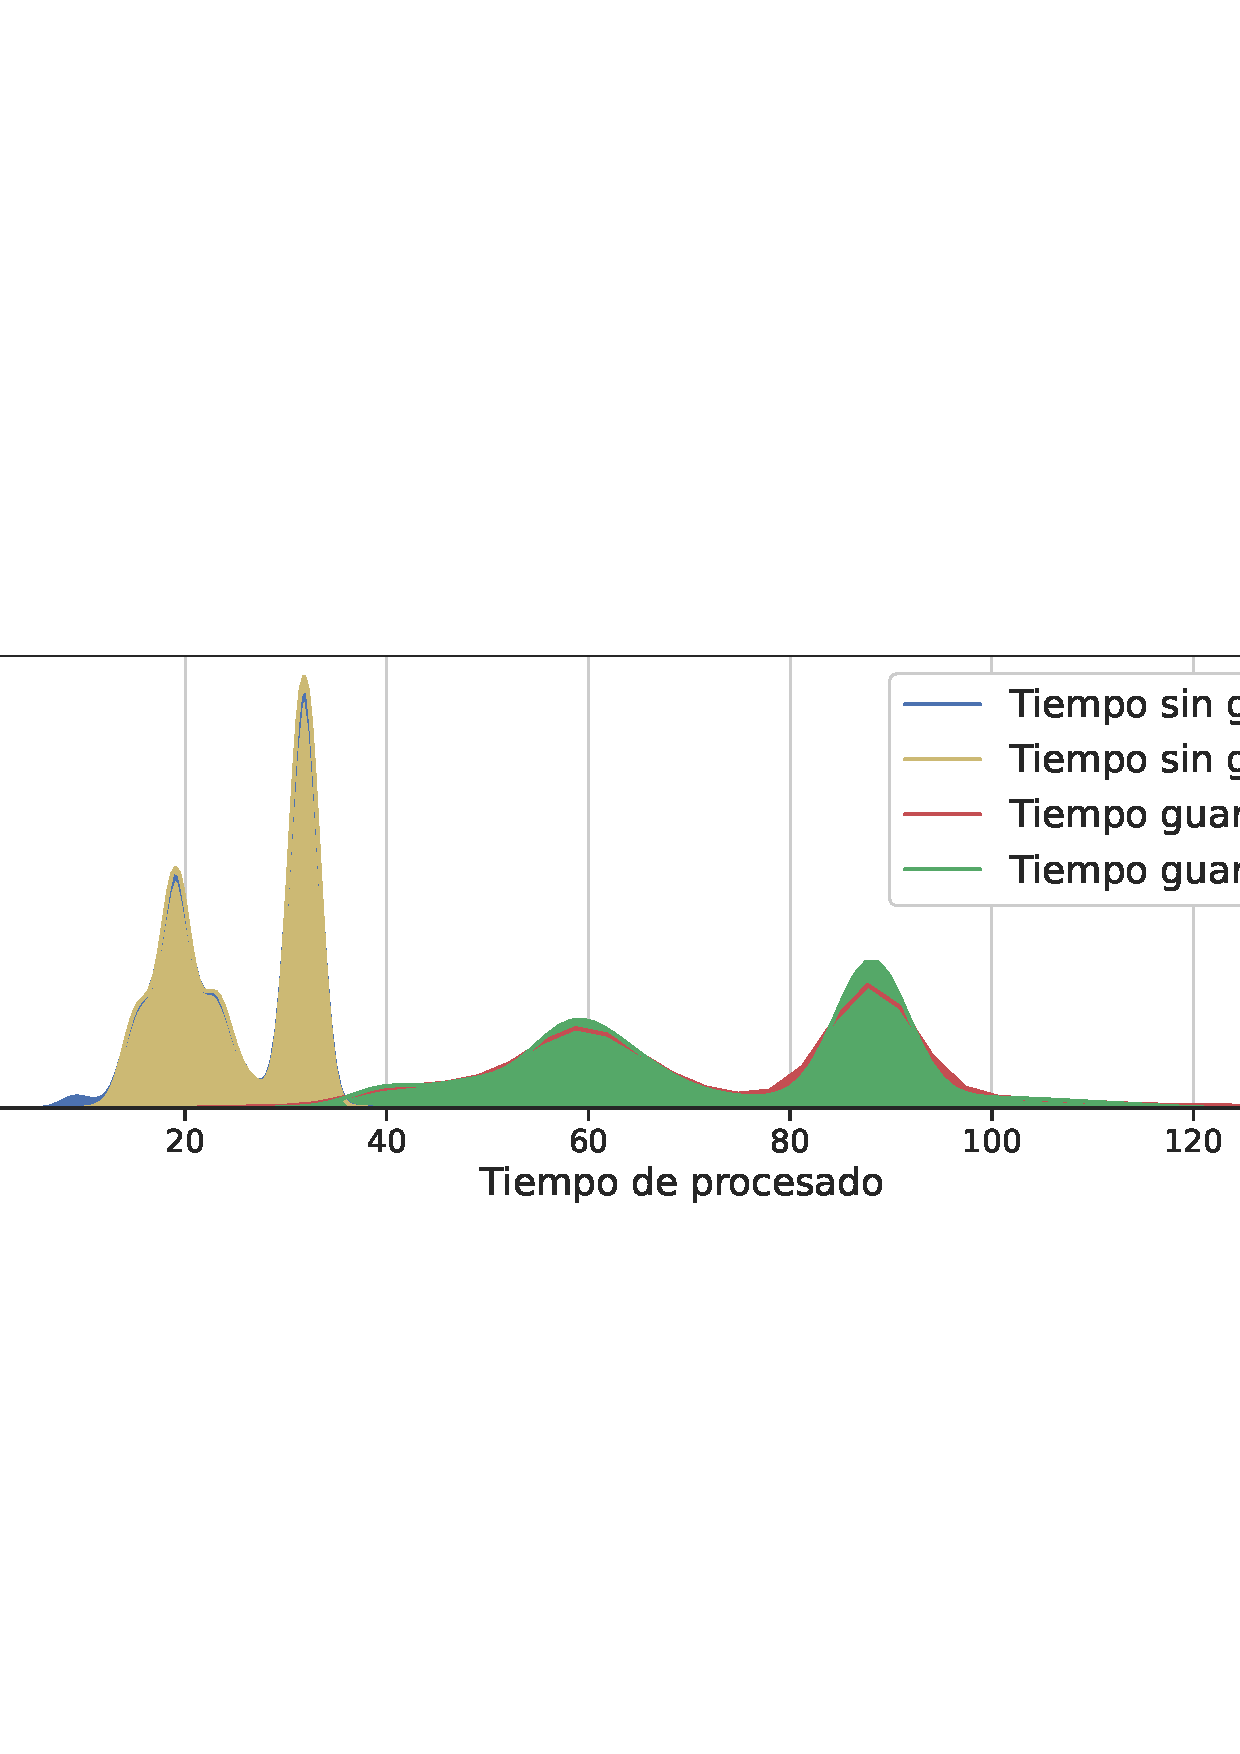
\includegraphics[width=\textwidth]{TiemposSinAccionDist.pdf}
		\caption{Imagen sin preprocesado.}
	\end{subfigure}
	\begin{subfigure}[b]{\textwidth}
		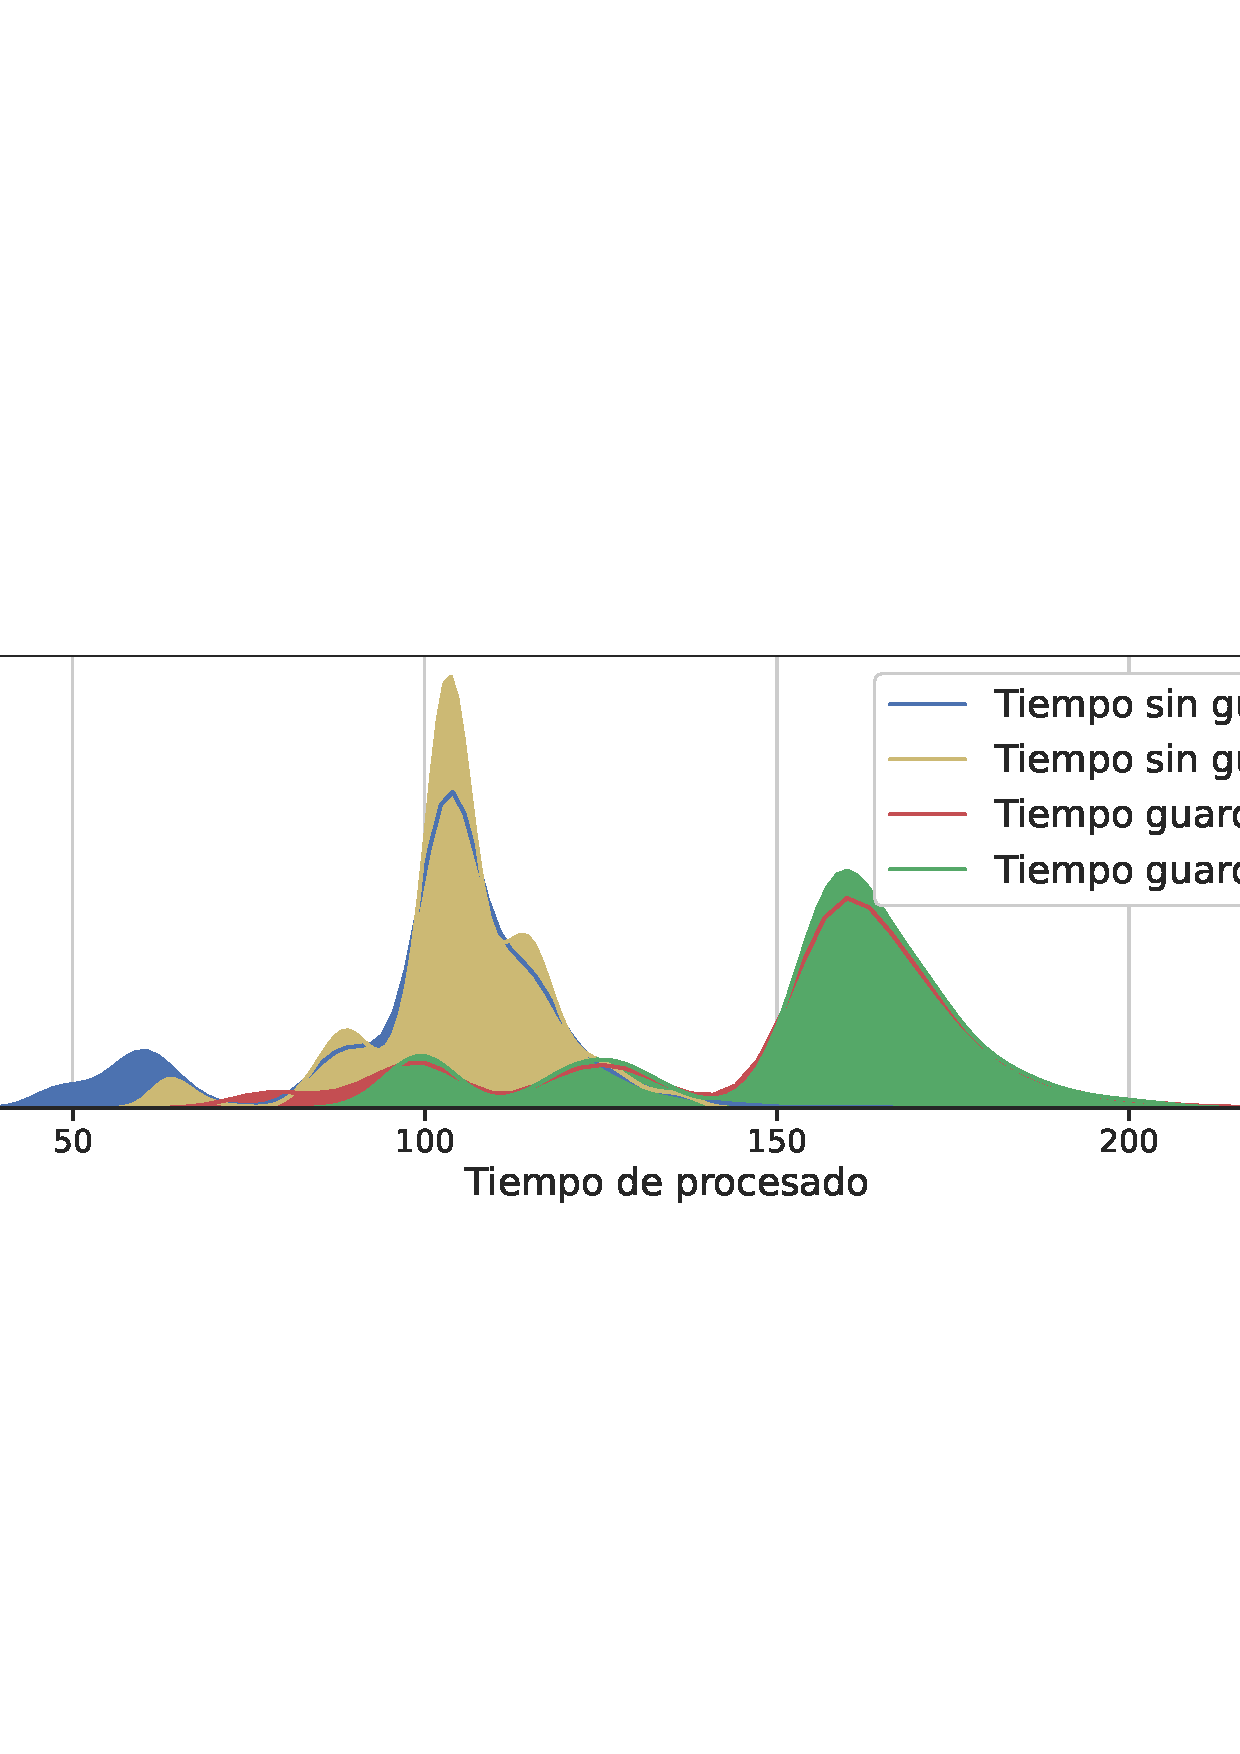
\includegraphics[width=\textwidth]{TiemposPrevioDist.pdf}
		\caption{Imagen con preprocesado.}
	\end{subfigure}
	\caption{Distribución de los datos temporales para el proceso del flujo sobre una imagen.}
	\label{fig:dist1}
\end{figure}


En la figura~\ref{fig:dist1} se pueden observar las distribuciones temporales para los casos considerados. La regla de las dos sigmas se cumple siempre con las distribuciones normales, sin embargo, aunque la distribución no es una normal si que asemeja su forma y abarca principalmente los datos temporales mayores por lo que se puede garantizar que el usar dos sigmas es suficiente rango temporal para el cálculo de \textit{workers}.

En la figura~\ref{fig:dist2} se observa la distribución estadística de los datos. Como es esperable el guardar las imágenes necesita de un tiempo considerablemente mayor. Los datos sin procesar la imagen son significativamente bajos, incluso la media sin guardar está en $17.5$ milisegundos, lo que alcanzaría un procesado de casi $60$ \textit{fps} para cada \textit{worker}. Son métricas muy buenas si se quiere extender el flujo que no necesiten la anonimización del rostro (como en cámaras de vigilizancia) o que ya vengan contrastadas. En el caso del preprocesado necesita de media $464$ milisegundos, que apenas da para procesar dos fotogramas por segundo.

\begin{figure}[h]
	\begin{subfigure}[b]{\textwidth}
		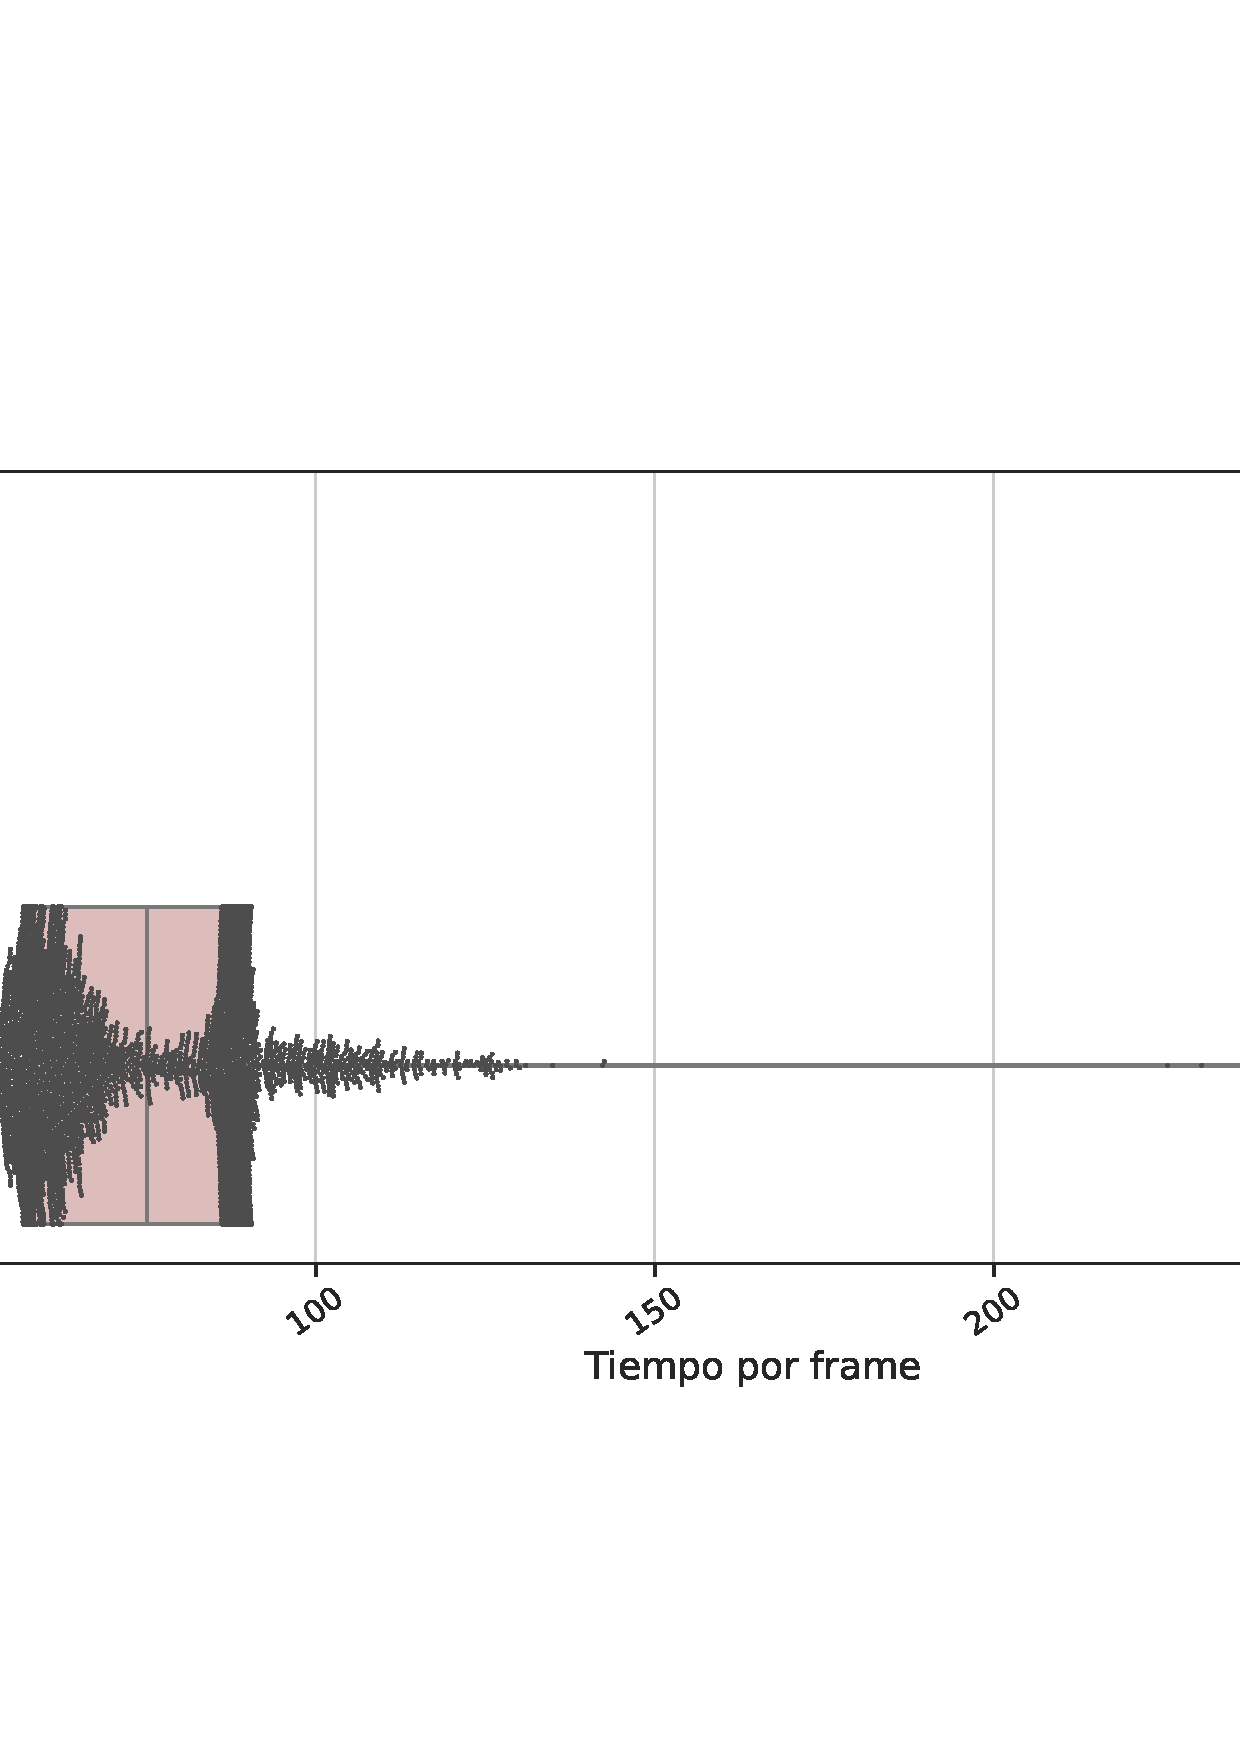
\includegraphics[width=\textwidth]{TiemposSinAccion.pdf}
		\caption{Imagen sin preprocesado.}
	\end{subfigure}
	\begin{subfigure}[b]{\textwidth}
		\includegraphics[width=\textwidth]{TiemposPrevio.pdf}
		\caption{Imagen con preprocesado.}
	\end{subfigure}
	\caption{Gráficos de bigotes con la distribución estadística de los datos temporales para el proceso del flujo sobre una imagen.}
	\label{fig:dist2}
\end{figure}

Con estos resultados, usando la \autoref{eq:fps}, podemos ver en la~\autoref{tab:workers1} la cantidad de \textit{workers} necesarios para ofrecer un procesado en tiempo real.

\begin{table}[h]
	\begin{center}
		\begin{tabular}{c  c c c c  }
			\toprule
			\multirow{2}{1.5cm}{\textbf{Tasa de \textit{fps}}}& \multicolumn{2}{c}{\textbf{Sin guardar}} & \multicolumn{2}{c}{\textbf{Guardando}}\\
			& \textbf{Sin procesar} & \textbf{Preprocesado} & \textbf{Sin procesar} & \textbf{Preprocesado}\\
			\otoprule
			\textbf{5 \textit{fps}} & 1 & 2 &1 & 3\\
			\textbf{15 \textit{fps}} & 1 & 1 &2 & 4\\
			\bottomrule
		\end{tabular}
	\end{center}
	\caption{N.º de \textit{workers} necesarios según el proceso a realizar.}
	\label{tab:workers1}
\end{table}


\subsection{Integración con el modelo de detección de esqueleto del paciente}

Se ha querido comprobar que la arquitectura de colas presentada en este trabajo funcionase correctamente en el proyecto que la engloba. Para ello se ha juntado con el modelo de clasificación para la detección del esqueleto y el cálculo de la diferencia entre dos estados.

Siguiendo las indicaciones\footnote{Ver \autoref{sec:manualpro}.} para hacer extensible el algoritmo, es decir, incorporar nuevas funcionalidades se ha incluido dentro del fichero \texttt{extraOpt.py} las importaciones de las clases creadas por José Miguel Ramírez Sanz, así como la instancia de la interfaz para acceder al modelo.

El primer detalle a tener en cuenta es que el modelo tenía que instanciarse en el ámbito global de la aplicación para que fuese serializado y enviado a todos los \textit{workers} de \textit{spark} ya que necesita para cargar entre 4 y 6 segundos, un tiempo excesivo que se sumaría al análisis de cada fotograma. Sin embargo, la inicialización del flujo necesita más tiempo por lo que es muy importante lanzarlo lo antes posible para cuando lleguen los primeros fotogramas esté completamente cargado.

Junto con la dificultad temporal surgió también una dificultar en memoria, concretamente la memoria de la tarjeta gráfica. Cada instancia cargada del modelo reservaba entre 512 y 768 MiB de VRAM por lo que según la cantidad de \textit{workers} se necesita una mayor cantidad de memoria en el sistema. En el caso personal, que se contaba con una \textit{Nvidia 750 Ti} de 2 GiB de memoria solamente se podían ejecutar un \textit{worker} junto con el \textit{master}, teniendo en cuenta la ecuación~\ref{eq:fps} implicaría que solamente se podían analizar $12$ en el caso de utilizar solamente el procesado básico y una tase de $3$ en el caso del flujo completo. Teniendo en cuenta las necesidades del tiempo real este dispositivo no es adecuado.

Al utilizar las GPU de la máquina \textit{gamma} del grupo \textit{ADMIRABLE}, que cuenta con tres \textit{Nvidia Titan Xp} de 12 GiB de memoria cada una se podían llegar a utilizar un total de 47 \textit{workers} junto con el nodo \textit{master}. Permitiendo así unas tasas de \textit{fps} de $288$ en el caso de solo usar el procesamiento básico y de $73$ con el flujo completo. Si los vídeos se mantienen con los \textit{15} fps se pueden tener $4$ flujos simultaneos y en el caso de reducir la tasa a 5 se pueden tener hasta $14$ flujos.


\subsection{Análisis temporal del flujo con toda la integración}\label{sec:analisistemporal}

Tal como se muestra en la \autoref{sec:analisistemporal_flujo} se realiza el mismo experimento con el flujo completo, es decir, se incorpora al preprocesado el modelo creado para este proyecto. En la \autoref{fig:boxplotTotal} se puede observar la distribución estadística de los datos evaluados. La media sin guardar la imagen es de $464$ ms y guardando de $626$ ms, las desviaciones típicas son de $86.5$ y $98.7$ respectivamente.

\begin{figure}[h]
	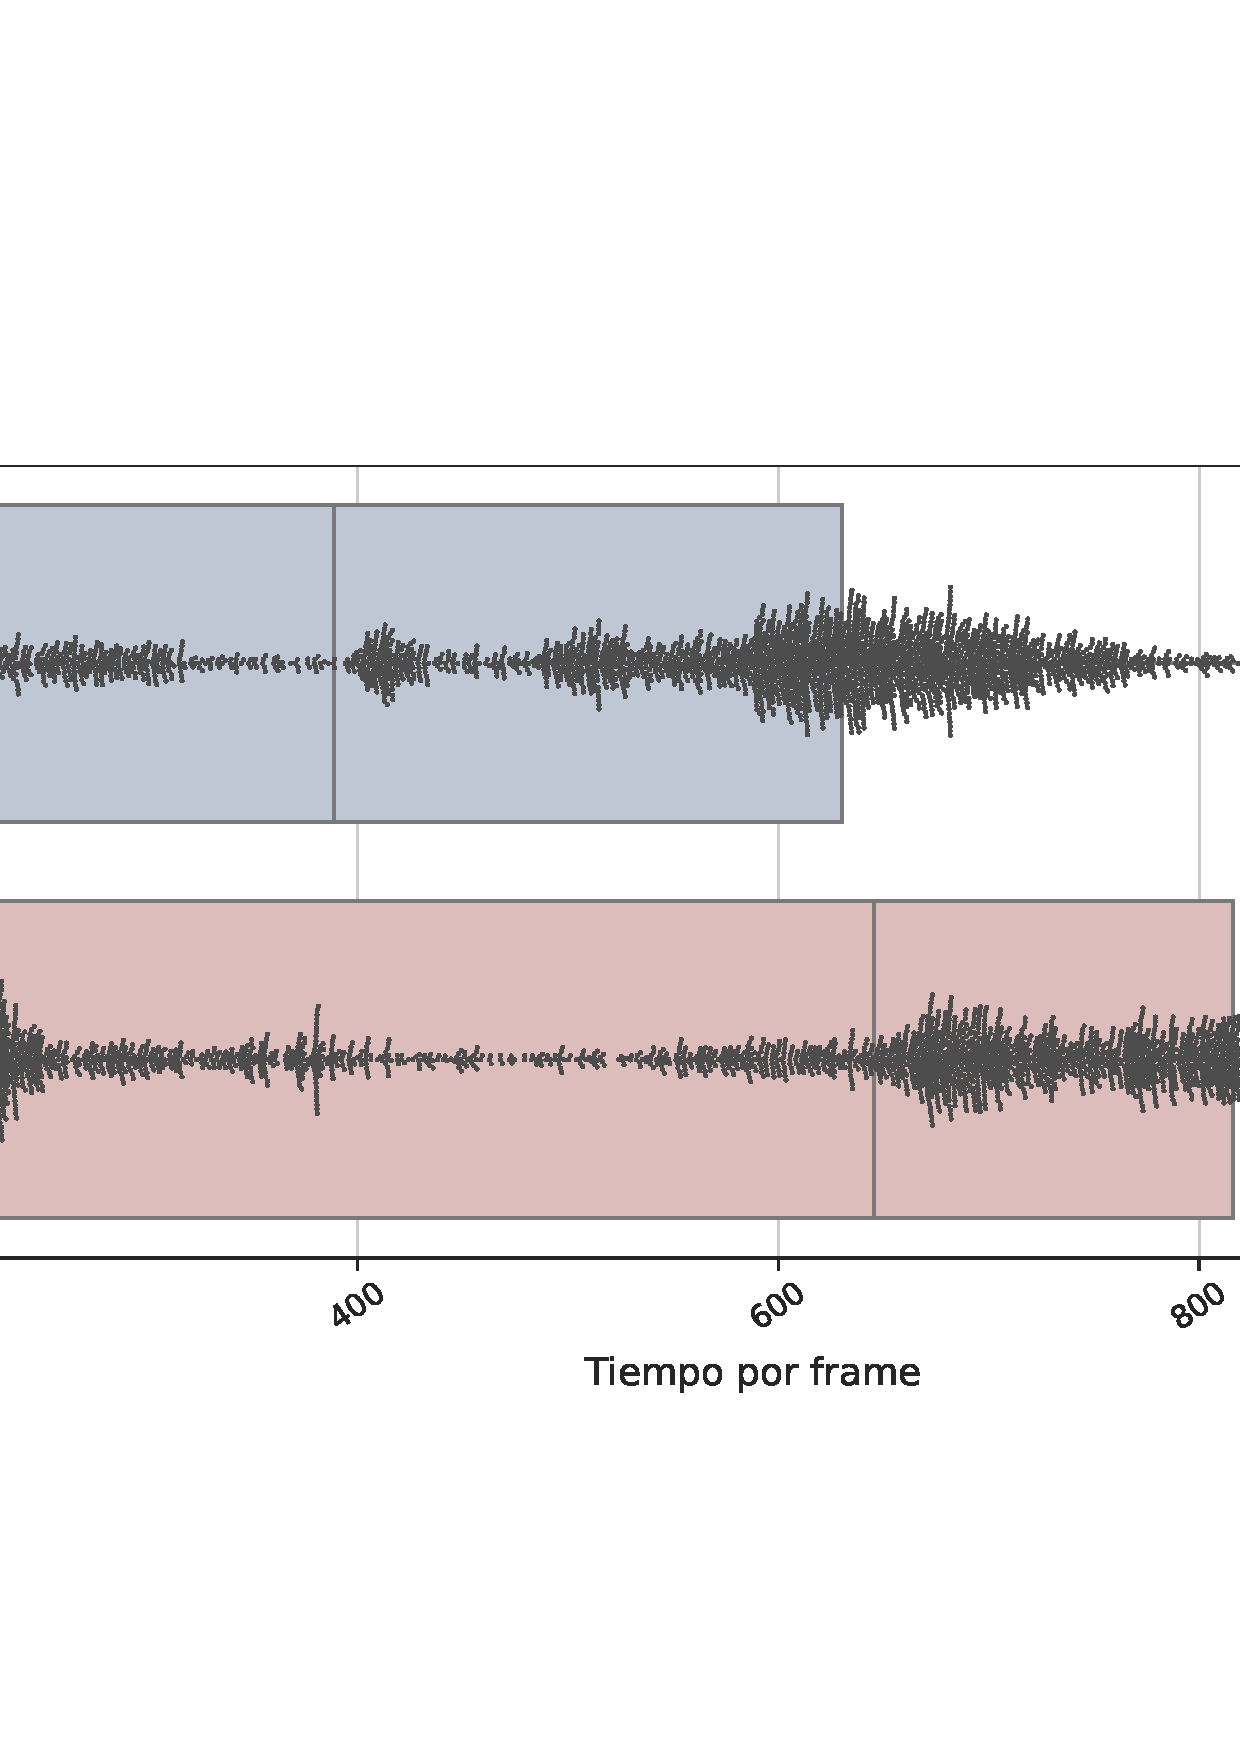
\includegraphics[width=\textwidth]{TiemposSumados.pdf}
	\caption{Gráficos de bigotes con la distribución estadística de los datos temporales para el proceso del flujo completo sobre una imagen.}
	\label{fig:boxplotTotal}
\end{figure}

Se necesitan, utilizando 15 \textit{fps} al menos 10 \textit{workers} si no se guarda y 13 en caso contrario. Por otro lado, de utilizar 5 \textit{fps} se necesitan 4 y 5 \textit{workers} sin guardar y guardando los fotogramas respectivamente.
\capitulo{6}{Trabajos relacionados}

Existe una literatura variada sobre técnicas para la rehabilitación de pacientes de la enfermedad del \textit{Parkinson} así como de aproximaciones para el análisis de vídeo en tiempo real. En este capítulo se expondrán algunos de los más relevantes.

\section{Literatura científica relacionada}

En el año 2019, Linares-del Rey \textit{et. al.}~\cite{linares2019aplicaciones} realizaron un meta-análisis sobre un total de veintiséis artículos de aplicaciones móviles para pacientes de \textit{Parkinson}. Se consideraron artículos en castellano y en inglés entre los años 2011 y 2016. Además se analizaron ciento y tres aplicaciones móviles que estuviesen en los principales \textit{marketplaces}: \textit{Google Play}, \textit{App Store} y \textit{Windows Store}.

El conjunto de estudios abarcaba a un total de cuatrocientos veinte pacientes y docientos treinta y dos personas sanas, estos como grupo de control en los artículos que los incluían. 

Para valorar la calidad metodológica de estos artículos se utilizó la escala JADAD~\cite{jadad1996assessing} basada en si existe o no aleatorización de los participantes, y se describe el método, si se hace un estudio de doble ciego, y se describe el método llevado para ello, y si se describen adecuadamente las pérdidas. Se suele tomar como valor mínimo aceptable una puntación de 3.

Entre el total de artículos revisados el único con una puntuación aceptable fue el sistema \textit{CuPid}~\cite{ginis2016feasibility} con un total de cuarenta participantes. La aplicación que presenta evaluaba la mejora de la calidad de vida del paciente según mejorasen su equilibrio, marcha y resistencia. Sin embargo, esta aplicación requería de uso de sensores externos al dispositivo móvil para poder evaluar la aplicación.

Respecto a las aplicaciones, al no tener artículos asociados (ya que de tenerlos se habrían analizado en el primer conjunto) no se podían evaluar siguiendo la misma escala. Sin embargo, algunas aplicaciones si que fueron analizadas por otras revisiones similares.

La conclusión de los autores fue que debido a la baja calidad metodológica y la poca cantidad de estudios realizados no se podía recomendar un uso generalizado de las aplicaciones, es decir, sigue haciendo falta la supervisar de terapeutas especializados que puedan dirigir y ayudar a la mejora de la calidad de vida de los pacientes.

\section{Aproximaciones en problemas similares}

El arquitecto de software Amit Baghel prensentó en 2016 una aproximación en Java para procesar vídeo utilizando \textit{Kafka} junto a \textit{Spark}~\cite{amit2017kafka}.

El objetivo de su trabajo era la creación de un detector de movimiento que combinase en una misma cola de \textit{Kafka} diferentes fuentes de vídeo y las procesase utilizando \textit{OpenCV} junto a \textit{Spark Streaming} y comparar cada \textit{frame} con el anterior y así detectar los objetos que se hubiesen movido.

\begin{figure}[h]
	\centering
	\includegraphics[width=1\textwidth]{amit}
	\caption[Diagrama de la arquitectura presentada por Amit Baghel.]{Diagrama de la arquitectura presentada por Amit Baghel. Fuente: \href{https://www.infoq.com/articles/video-stream-analytics-opencv/}{Infoq}}
\end{figure}

Debido a la similitud de la arquitectura de este trabajo con la que se deseaba contruir se utilizó como base en algunas decisiones del diseño. Concretamente se decidió mantener la configuración planteada para \textit{Kafka}: cantidad de particiones  en tres y el factor de replicación de uno.

Sin embargo, la arquitectura presentada, debido a los cambios de las versiones del los últimos años, ya no se puede desplegar en los sistemas \textit{GNU/Linux} modernos a menos que se compilen directamente las versiones que plantean.
\capitulo{7}{Conclusiones y Líneas de trabajo futuras}

Para finalizar la exposición de esta memoria se comentará en este capítulo las conclusiones del 
trabajo así como líneas futuras que se van a realizar.

\section{Conclusiones}

De este trabajo se han sacado diversas conclusiones:

\begin{itemize}
	\item Las herramientas que ofrece la \textit{suite} \textit{Apache} para la gestión y procesado de flujo son muy robustas y tiene el desempeño que se espera de ellas, especialmente referente a la flexibilidad y fiabilidad. Sin embargo, existen aún muchas limitaciones en la documentación que en muchas ocasiones es muy <<esotéricas>>, especialmente a la hora de enseñar a integrar las diversas tecnologías. De hecho, una de las mayores dificultades encontradas para el cumplimiento de los objetivos ha sido la integración correcta de las herramientas.
	\item Los objetivos del proyecto han sido cumplidos al completo, habiendo conseguido tanto una aplicación sencilla para comunicar a pacientes y usuarios como también una arquitectura fundada sobre una tecnología robusta para facilitar el análisis en tiempo real. Se espera que esto conlleve una mejora continua de la calidad de vida de los pacientes de la enfermedad de \textit{Parkinson} al tener un acceso más fácil a los profesionales de la terapia ocupacional.
\end{itemize}

\section{Lineas futuras}

Dentro de las lineas futuras están:

\begin{itemize}
	\item Integrar el flujo con la aplicación de \textit{Jitsi} para que funcione automáticamente con los pacientes.
	\item Desplegar su uso con terapeutas y pacientes reales a una mayor escala. Actualmente se tiene un único paciente y terapeuta, pero el objetivo a largo plazo es que la herramienta se pueda usar por una cantidad mayor de personas.
	\item Automatizar el despliegue en clúster de servidores utilizando \textit{Kubernetes}~\cite{losautoresdekubernetes2020}, herramienta creada por \textit{Google} que permite la creación fácil de un clúster de máquinas virtuales \textit{Docker} lo que permetiría una mayor versatilidad sobre los \textit{scripts} creados en este trabajo.
	\item Explorar mejores configuraciones para \textit{Kafka} y \textit{Spark Streaming} para mejorar el desempeño del flujo.
\end{itemize}


%\renewcommand\chaptername{Anexo}
%\renewcommand\thechapter{\Roman{chapter}}
%\setcounter{chapter}{0}

% Añadir entrada en el índice: Anexos
\appendix
\addcontentsline{toc}{part}{Apéndices}
\part*{Apéndices}

\apendice{Plan de Proyecto Software}

\section{Introducción}

En este apéndice se expondrán los distintos \textit{sprints} que se han realizado y un estudio de la viabilidad del proyecto.

\section{Planificación temporal}

La planificación temporal se ha realizado adaptando la metodología \textit{Scrum}. Para poder adaptarlo a un trabajo de una sola persona para un proyecto educativo se han considerado las siguientes indicaciones:

\begin{itemize}
	\item El desarrollo se ha basado en iteraciones o \textit{sprints} de dos semana de duración aproximadamente.
	\item Cada uno de los \textit{sprints} contiene las tareas que se realizaron en el mismo. 
	\item Cada tarea tiene un coste estimado dependiendo de lo que el programador estime conveniente siguiendo los parámetros de tiempo a emplear, dificultad técnica entre otros.
	\item Una vez concluida una tarea se especifica el coste real para poder estimar de una manera más correcta tareas de \textit{sprints} siguientes.
	\item Al finalizar cada \textit{sprint} se realiza una reunión con los tutores del proyecto.
\end{itemize}

\subsection{Sprint 0}

El \textit{sprint} 0 consistió en el desarrollo de la aplicación web para la recogida de datos para el proyecto. Es el único \textit{sprint} realizado en colaboración con el alumno José Miguel Ramírez Sanz. 

\begin{table}[H]
	\begin{tabularx}{\linewidth}{X r r}
		\toprule \textbf{Tarea} & \textbf{Est.} & \textbf{Final}\\
		\otoprule
		Diseño de la interfaz web & 3 & 3 \\
		Creación de la plantilla maestra de toda la web & 3 & 2 \\
		Creación de la plantilla base para el menú del paciente & 5 & 5 \\
		Implementación del menú del terapeuta & 2 & 2 \\
		Creación de la conexión para videollamada - Terapeuta & 1 & 1 \\
		Creación de la conexión para videollamada - Paciente & 1 & 1 \\
		Implementación del sistema de inicio de sesión & 2 & 3 \\
		Creación de \textit{plugin} para la captura y emisión del vídeo del paciente & 8 & 13 \\
		Creación de la interfaz de gestión del paciente  & 2 & 2	\\	
		\bottomrule
	\end{tabularx}
	\caption{Tareas del \textit{sprint} 0}
	\label{tab:sprint0}
\end{table}

La mayor dificultad en este \textit{sprint} fue la creación del \textit{plugin} sobre \textit{Jitsi} que duplicase el flujo de vídeo y emitiese los datos del servidor al sistema de colas. Esto fue debido a la poca documentación de \textit{Jitsi} sobre la implantación de estas modificaciones. 


\subsection{Sprint 1}

El \textit{sprint} 1 consistió en la exploración de herramientas para la creación y procesado de flujos de vídeo. 

\begin{table}[H]
	\begin{tabularx}{\linewidth}{X r r}
		\toprule \textbf{Tarea} & \textbf{Est.} & \textbf{Final}\\
		\otoprule
		Búsqueda de herramientas para la creación de flujos de datos & 3 & 3 \\
		Pruebas sobre \textit{Apache Flume} & 5 & 3 \\
		Pruebas sobre \textit{Apache Kafka} & 5 & 5 \\
		Búsqueda de herramientas para el despliegue por contenedores & 3 & 3 \\
		Prueba de despliegue de \textit{Apache Kafka} para \textit{Docker} & 3 & 3 \\
		Búsqueda de herramientas para el procesado de flujos de vídeo & 3 & 3 \\
		Pruebas con \textit{Spark Streaming} con \textit{OpenCV} & 5 & 13 \\
		\bottomrule
	\end{tabularx}
	\caption{Tareas del \textit{sprint} 1}
	\label{tab:sprint1}
\end{table}

El desarrollo de este \textit{sprint} fue bastante similar a lo planificado. El caso particular estuvo en la última tarea debido a la complejidad conectar y procesar de manera efectiva \textit{Spark Streaming} con la librería de OpenCV y poder garantizar que no se perdían \textit{frames.}

\subsection{Sprint 2}

El \textit{sprint} 2 consistió en la implementación de las conexiones entre todos los elementos del flujo a nivel local. 

\begin{table}[H]
	\begin{tabularx}{\linewidth}{X r r}
		\toprule \textbf{Tarea} & \textbf{Est.} & \textbf{Final}\\
		\toprule
		Despliegue local de \textit{Apache Spark} & 2 & 2\\
		Despliegue local de \textit{Apache Kafka} & 3 & 5\\
		Simulación de servidor UDP para vídeo & 5 & 5 \\
		Ingestor a Kafka del vídeo UDP & 3 & 5\\
		Conectar \textit{Spark Streaming} con \textit{Kafka}& 3 & 13\\
		Implementar un anonimizador de rostros & 3 & 2\\
		Parametrizar todos los \textit{scripts} creados & 2 & 2	\\
		\bottomrule
	\end{tabularx}
	\caption{Tareas del \textit{sprint} 2}
	\label{tab:sprint2}
\end{table}

La razón de la gran diferencia en la quinta tarea del \textit{sprint} entre predicho e invertido fue debido a que la documentación de \textit{Kafka} no estaba bien detallada para conectar con \textit{Spark Streaming}. 

\subsection{Sprint 3}

El \textit{sprint} 3 consistió en la implementación de una infraestructura de contenedores \textit{Docker} que conectase todos los servicios para el flujo. 

\begin{table}[H]
	\begin{tabularx}{\linewidth}{X r r}
		\toprule \textbf{Tarea} & \textbf{Est.} & \textbf{Final}\\
		\otoprule
		Despliegue de \textit{Apache Spark} para el nodo \textit{master} & 2 & 2\\
		Despliegue de \textit{Apache Spark} para varios nodos \textit{worker} & 2 & 1\\
		Creación de imágenes \textit{Docker} para soportar las aplicaciones creadas & 8 & 21\\
		Despliegue de la aplicación \textit{openCV} & 3 & 3 \\
		Recogida de \textit{stream} de vídeo e ingestión en \textit{Kafka} en \textit{Docker} & 8 & 8\\
		\bottomrule
	\end{tabularx}
	\caption{Tareas del \textit{sprint} 3}
	\label{tab:sprint3}
\end{table}

Este \textit{sprint} fue más sencillo que el anterior, principalmente porque en el anterior existieron dificultades para cumplir con los plazos del mismo al complicarse la tarea de conectar dos de los componentes. Con la experiencia obtenida en ese \textit{sprint} algunas tareas se desarrollaron más fácilmente. Por otro lado el despliegue con \textit{docker} necesitó casi un \textit{sprint} aparte ya que muchas de las operaciones, a \textit{priori} simples, resultaron tener varias capas de complejidad no previstas. Esto causó el mayor desajuste entre lo previsto y lo invertido de todo el proyecto, presumiblemente por la poca experiencia previa en el uso de contenedores \textit{docker}.

\subsection{Sprint 4}

El \textit{sprint} 4 consistió en la automatización de los procesos del \textit{sprint} 3. 

\begin{table}[H]
	\begin{tabularx}{\linewidth}{X r r}
		\toprule \textbf{Tarea} & \textbf{Est.} & \textbf{Final}\\
		\otoprule
		\textit{Script} para la creación de \textit{topics} de \textit{Kafka} & 1 & 1\\
		\textit{Script} de lanzamiento de instancia del flujo & 8 & 13 \\
		\textit{Script} de inicialización de los servicios & 2 & 2\\
		\textit{Script} para la eliminiación de un \textit{topic} de \textit{Kafka} & 1 & 1\\
		\textit{Script} para el cierre ordenado de un flujo & 5 & 8\\
		\textit{Script} para el apagado completo de los servicios & 1 & 1\\
		\bottomrule
	\end{tabularx}
	\caption{Tareas del \textit{sprint} 4}
	\label{tab:sprint4}
\end{table}

La mayor dificultad de este \textit{sprint} estuvo en la creación de los \textit{scripts} que abarcasen tanto el inicio como el cierre de un flujo debido a que estaban involucrados tanto el inicio de las imágenes \textit{docker} asociadas, el control de identificadores (realizado mediante semáforos en forma de ficheros) y la ejecución ordenada. Por estos motivos las predicciones no fueron acertadas al complicarse la implementación.

\subsection{Sprint 5}

El \textit{sprint} 5 consistió en la creación de experimentos para evaluar el tiempo necesitado para el procesado del flujo además de la búsqueda de un sistema de serialización y compresión adecuado para el encolado de los fotogramas. 

\begin{table}[H]
	\begin{tabularx}{\linewidth}{X r r}
		\toprule \textbf{Tarea} & \textbf{Est.} & \textbf{Final}\\
		\toprule
		Diseño de los experimentos & 3 & 3\\
		Implementación de los experimentos del flujo & 5 & 13\\
		Implementación de los experimentos sobre las técnicas de serialización y compresión & 5 & 5\\
		Implementación de la recogida y visualización de los resultados & 3 & 3\\
		Análisis de los resultados & 3 & 3\\
		\bottomrule
	\end{tabularx}
	\caption{Tareas del \textit{sprint} 5}
	\label{tab:sprint5}
\end{table}

Hubo una gran dificultad a la hora de la implementación de los experimentos debido a que se quiso paralelizar la ejecución y acelerar así el proceso. Sin embargo, esto conllevó un estudio más en profundidad de las herramientas de \textit{Python} para ello.

\subsection{Sprint 6}

En este penúltimo \textit{sprint} se comenzó el despliegue real y la integración con el modelo predictivo de poses del alumno José Miguel Ramírez Sanz. 

\begin{table}[H]
	\begin{tabularx}{\linewidth}{X r r}
		\toprule \textbf{Tarea} & \textbf{Est.} & \textbf{Final}\\
		\toprule
		Implementación de la extensibilidad del flujo & 2 & 2\\
		Instalación local del flujo completo & 3 & 3\\
		Instalación de las librerías necesarias en el equipo \textit{Gamma} & 1 & 1\\
		Despliegue de las máquinas \textit{docker} en \textit{Gamma} & 1 & 1\\
		Pruebas sobre vídeos pregrabados & 2 & 2\\
		Adaptación de los \textit{dockers} para compatibilidad con \textit{Nvidia} & 8 & 13\\
		Diseño de experimentos sobre el flujo completo & 1 & 1\\
		Implementación de los experimentos & 8 & 5\\
		Análisis de los resultados & 2 & 2\\
		\bottomrule
	\end{tabularx}
	\caption{Tareas del \textit{sprint} 6}
	\label{tab:sprint6}
\end{table}

El \textit{sprint} se desarrolló con bastante facilidad respecto a otros debido principalmente a que gran parte del material necesario, como los \textit{scripts} de lanzamiento o experimentos similares, ya se habían creado anteriormente. El único problema estuvo relacionado con la adaptación de las imágenes \textit{Docker} a \textit{Nvida} ya que se requirieron muchos cambios inesperados para que funcionase adecuadamente.

\subsection{Sprint 7}

Este último \textit{sprint} consistió en la creación de la documentación del trabajo realizado. 

\begin{table}[H]
	\begin{tabularx}{\linewidth}{X r r}
		\toprule \textbf{Tarea} & \textbf{Est.} & \textbf{Final}\\
		\otoprule
		Maquetación de la plantilla & 1 & 1\\
		Escritura de la introducción & 2 & 2\\
		Escritura de los objetivos & 3 & 3\\
		Escritura de los conceptos teóricos & 5 & 5\\
		Escritura de los aspectos relevantes & 13 & 13\\
		Escritura de los trabajos relacionados & 3 & 3\\
		Escritura de las conclusiones y lineas futuras & 2 & 2\\
		Escritura del plan de proyecto & 2 & 2\\
		Escritura del diseño & 5 & 5\\
		Escritura del manual del programador & 3 & 3\\
		Creación de la presentación & 8 & 8\\  
		\bottomrule
	\end{tabularx}
	\caption{Tareas del \textit{sprint} 7}
	\label{tab:sprint7}
\end{table}


\section{Estudio de viabilidad}


\subsection{Viabilidad económica}

Debido a que este TFM está dentro de un proyecto donde también se encuentra el TFM de José Miguel Ramírez Sanz, se ha realizado el estudio de viabilidad económica de manera conjunta


En la \autoref{tab:costes_personal} se encuentran los costes total en salarios en jornada completa durante seis meses para dos empleados.

\begin{table}[H]\centering
	\begin{tabular}[]{@{}l r@{}}
		\toprule
		\textbf{Concepto} & \textbf{Coste (\euro{})} \\
		\midrule
		Salario mensual bruto~\cite{salariales} & 2\,047,78 \\
		Seguridad Social (30,04\%) & 615,15 \\
		Retención IRPF (2\%) & 28,65 \\
		Salario mensual neto & 1\,403,97 \\\hubu
		\textbf{Total 6 meses y dos empleados} &  24\,573,36 \\
		\bottomrule
	\end{tabular}
	\caption{Costes de personal.}
	\label{tab:costes_personal}
\end{table}

La \autoref{tab:costes_hardware} están las inversiones y amortizaciones  en materia de \textit{hardware}, tanto los \textit{MainFrames} para el despliegue y el cálculo como los equipos de desarrollo.


\begin{table}[H]
	\centering
	\begin{tabular}[]{@{}l r r@{}}
		\toprule
		\textbf{Concepto} & \textbf{Coste (\euro{})} & \textbf{Coste amortizado (\euro{})} \\
		\otoprule
		Ordenador de desarrollo (x2) & 950 &  59,37\\
		Dispositivos pacientes (x9) & 100 & 6,25\\
		\textit{Webcam} pacientes (x9) & 150 &9,38\\
		\textit{MainFrame Gamma}  & 3\,000 & 187,5 \\ 
		\textit{Gamma} GPU (x3) & 1\,500 &  93,75\\
		\textit{MainFrame Alpha}  & 2\,000 & 125 \\\hubu
		\textbf{Total} & 13\,650 & 853,16\\
		\bottomrule
	\end{tabular}
	\caption{Costes de \textit{hardware}.}
	\label{tab:costes_hardware}
\end{table}

Por último en la \autoref{tab:costes_servicios} se encuentran los dos servicios contratados para dar acceso a la aplicación a los pacientes.

\begin{table}[H]
	\centering
	\begin{tabular}[]{@{}l r@{}}
		\toprule
		\textbf{Servicio} & \textbf{Coste (\euro{})}\\
		\otoprule
 		Suscripción \textit{Ngrok}  & 7,33 \\
		Lineas \textit{Vodafone} (x4) & 30 \\\hubu
		\textbf{Total (por 6 meses)} & $763.68$\\
		\bottomrule
	\end{tabular}
	\caption{Costes de servicios.}
	\label{tab:costes_servicios}
\end{table}

Los costes totales se pueden observar en la \autoref{tab:costes_totales}.

\begin{table}[H]
	\centering
	\begin{tabular}[]{@{}l r@{}}
		\toprule
		\textbf{Servicio} & \textbf{Coste (\euro{})}\\
		\otoprule
		Costes de personal  & 24\,573,36 \\
		Costes de \textit{hardware} & 13\,650 \\
		Costes de servicios & $763.68$ \\\hubu
		\textbf{Total} & 38\,987,04\\
		\bottomrule
	\end{tabular}
	\caption{Costes totales.}
	\label{tab:costes_totales}
\end{table}


\subsection{Viabilidad legal}

Este proyecto se ha realizado con la ayuda de software de terceros con licencias propias que influyen sobre la viabilidad legal del proyecto.

Dentro de las licencias de las herramientas utilizadas están:
\begin{itemize}
		\item \textbf{MIT}: Esta licencia permite el uso comercial del producto, la modificación del mismo, la libre distribución y el uso privado. No tiene garantías ni responsabilidad. La única condición es hacer referencia a ella. Como no obliga a mantener la licencia ni afecta a la distribución del software que use la licencia final del producto, esta puede ser cualquiera.
		
		\item \textbf{GPLv3}: Licencia que permite uso comercial, distribución, modificación uso privado y creación de patentes. Obliga a licenciar
cualquier modificación del código o códigos que usen herramientas con esta licencia usar \textbf{GLPv3} u otras versiones.
		
		\item \textbf{Apache 2.0}: Licencia de las herramientas de Apache, tiene las mismas propiedades que la licencia GPLv3 con excepción de que no obliga a que las nuevas implementaciones con dependencias en Apache 2.0 sean licenciadas como código libre.

		\item \textbf{BSD}: Tiene características semejantes a MIT en el contexto en el que la usamos.
		
		\item \textbf{BSD 3-Clause}: Tiene características semejantes a MIT en el contexto en el que la usamos.
\end{itemize}

La licencia más restrictiva del proyecto, la \textit{GPLv3}, está asociada a las plantillas de imágenes \textit{docker} de Mario Juez Gil~\cite{juez2019docker}. Como el resto de licencias son compatibles con la \textit{GPLv3} se utiliza dicha licencia para todo el proyecto.

\subsubsection{\textit{Copyright} de terceros}

\textbf{Apache 2.0}:
\begin{itemize}
	\item \textit{Apache Kafka} - \textit{Apache Foundation}
	\item \textit{Apache Zookeeper} - \textit{Apache Foundation}
	\item \textit{Apache Spark} - \textit{Apache Foundation}
	\item \textit{Docker CP} - \textit{Confluentic}
	\item \textit{Jitsi Meet} - \textit{Jitsi}
\end{itemize}

\textbf{GPLv3}:
\begin{itemize}
	\item \textit{Clúster Spark Docker} - Mario Juez Gil
\end{itemize}

\textbf{BSD} todas sus variantes:
\begin{itemize}
	\item \textit{Caffe} - \textit{BVLC}
	\item \textit{Flask} - \textit{Pallets}
	\item \textit{Jinja} - \textit{Pallets}
	\item \textit{OpenCV} - \textit{Intel Corporation}, \textit{Xperience AI}
	\item \textit{Seaborn} - Michael Waskom
\end{itemize}

\textbf{MIT}
\begin{itemize}
	\item \textit{Bootstrap 4} - \textit{Twitter}
	\item \textit{jQuery} - \textit{JS Foundation}
\end{itemize}


%\apendice{Especificación de Requisitos}

Este apartado no se como afrontarlo realmente porque los objetivos generales creo que están descritos en los objetivos del proyecto y el catálogo de requisitos y su especificación está más orientado a casos de uso.
\section{Introducción}

\section{Objetivos generales}

\section{Catalogo de requisitos}

\section{Especificación de requisitos}



\apendice{Especificación de diseño}

\section{Introducción}

El sistema completo funciona con la unión de dos subsistemas. El subsistema web que lo forman el servidor que identifica al usuario y la plataforma \textit{Jitsi} para realizar la videollamada y el subsistema de colas, que da nombre a este trabajo, que encola los \textit{frames} del vídeo y los procesa. 

En este apartado se explica como se ha diseñado el sistema completo, la comunicación entre todas sus partes, el flujo del trabajo y la composición de cada elemento.

\section{Diseño procedimental}

El procedimiento para el procesado de los vídeos (\autoref{fig:secuencias}) para cada paciente que entre en una videollamada (independientemente de que esté o no el terapeuta) se inicializa un nuevo \texttt{Ingestor} que encolará los frames que reciba. A su vez este \texttt{Ingestor} creará un procesador que consumirá los \textit{frames} y los procesará. Estos dos elementos permanecerán hasta que sean cerrados por la finalización de la conexión. Por tanto, por cada paciente conectado se procesará tan pronto como sea posible la secuencia de \textit{frames} del mismo.

\begin{figure}
	\centering
	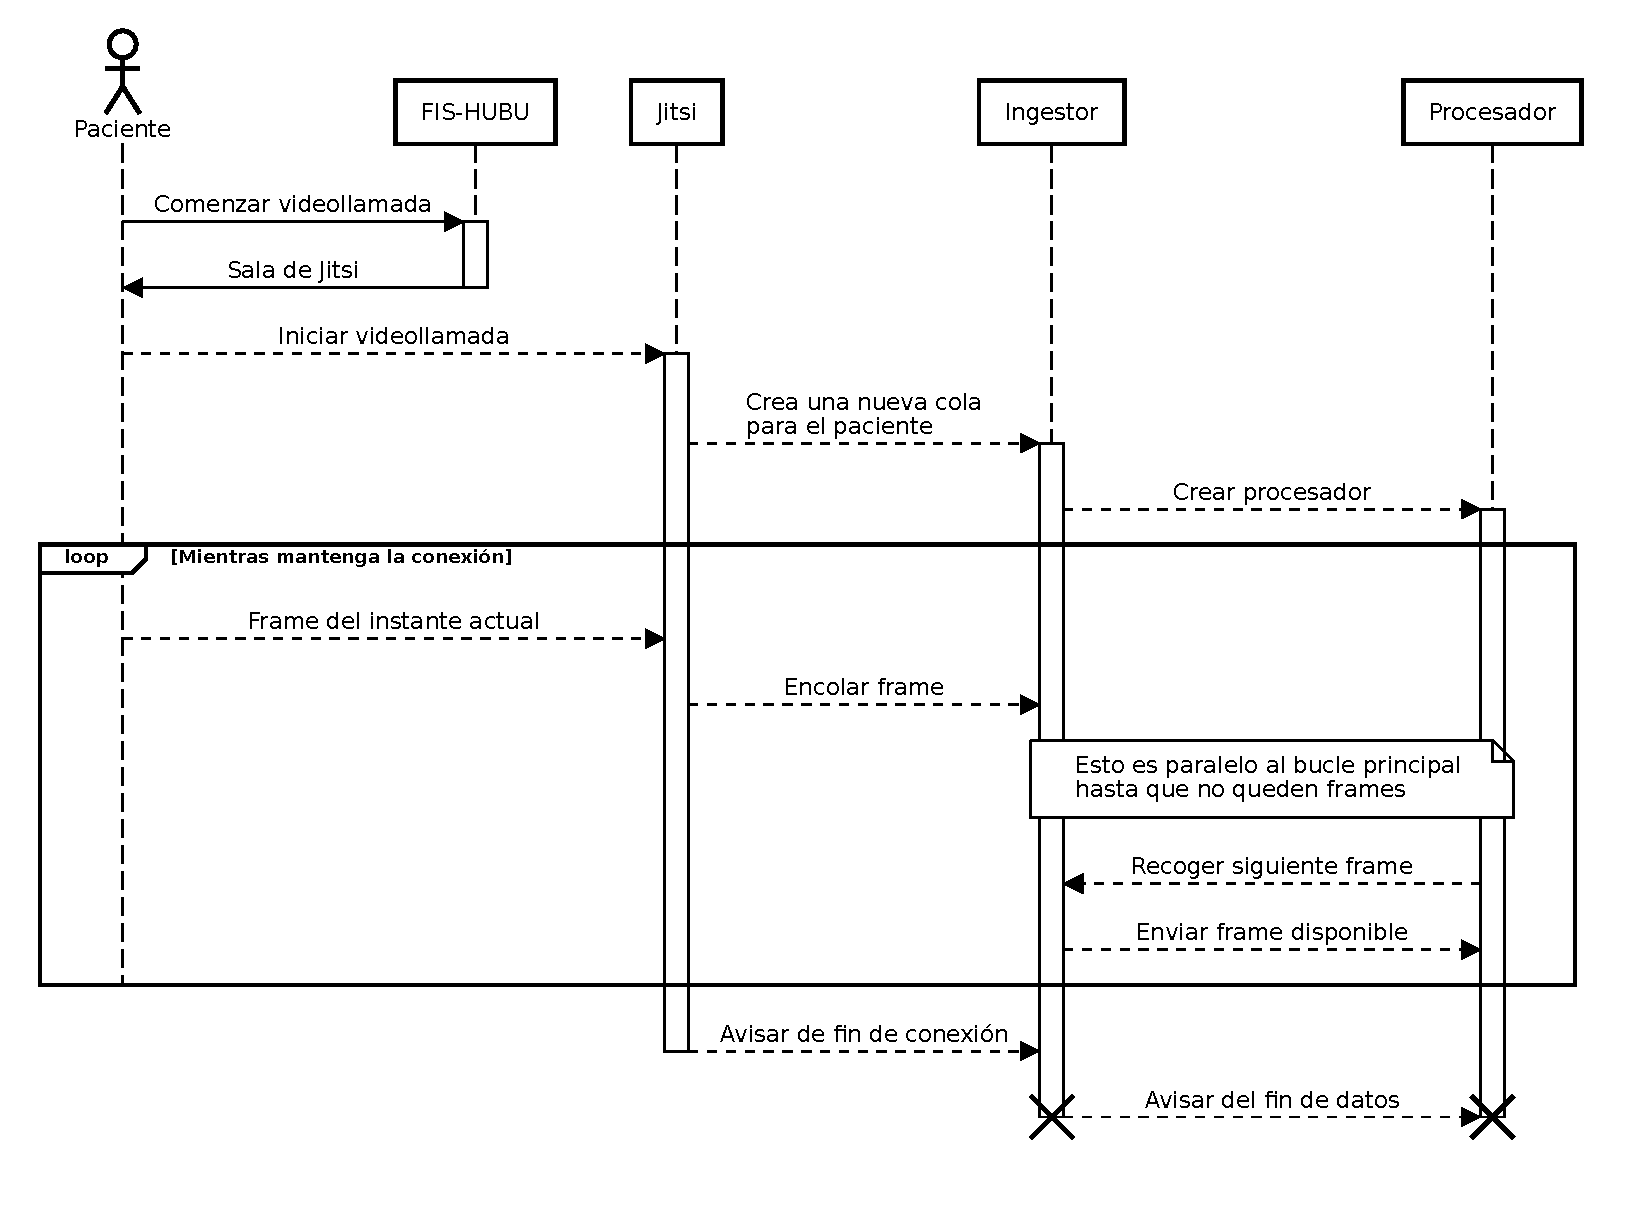
\includegraphics[width=\textwidth]{Secuencias}
	\caption[Diagrama de secuencia para el proceso general de la aplicación.]{Diagrama de secuencias para el proceso general de la aplicación. Conexión del paciente y procesado del vídeo de entrada.}
	\label{fig:secuencias}
\end{figure}



\section{Diseño arquitectónico}

La parte más esencial de este trabajo es la creación del \textit{pipeline} que procesa en tiempo real los \textit{frames} de la comunicación del paciente. Todo ello se ha desarrollado, utilizando las herramientas de la suite de \textit{Apache}, \textit{Apache Kafka} para el \textit{ingestor}, \textit{Apache Spark Streaming} para el \textit{procesador}. En la \autoref{fig:flujoetlreal} se puede observar el funcionamiento completo del flujo y las partes que lo componen.

Para que esta arquitectura sea ajena al entorno se encapsulan sobre máquinas virtuales \textit{Docker} de tal forma que se pueda desplegar en cualquier sitio. Concretamente habría cuatro tipos de imágenes \textit{Docker}. La primera se encarga de la serialización de los frames y lanzan el \textit{script} de \textit{Python} de encolado, esta máquina se crea y destruye a voluntad de las conexiones de los pacientes. La segunda y tercera imagen es el servicio de \textit{Zookeeper} y de \textit{Kafka}. Estas imágenes no se duplican en caso de cambios en las conexiones, unicamente se crean o borran colas. Por último, la cuarta imagen es la transformación del flujo. Se crean o se destruyen según las conexiones de los pacientes y se parametrizan para que consuman un flujo concreto y hagan un procesamiento concreto de tal forma que diferentes pacientes se podrían configurar para tener diferentes procesados permitiendo una mayor flexibilidad en el procesamiento.

\begin{figure}[H]
	\centering
	\includegraphics[width=\textwidth]{Flujo-FIS-HUBU}
	\caption[Implementación del flujo ETL para el procesado de imágenes en tiempo real.]{Implementación del flujo ETL para el procesado de imágenes en tiempo real. Por cada paciente conectado se asocia a un \textit{ingestor} que serializa la imagen y la encola en un flujo de \textit{Apache Kafka} dividido en tres particiones. Cada cola es procesada por un servidor de \textit{Apache Zookeeper}. El flujo es consumido por un procesador de \textit{Apache Spark Streaming}. El procesado puede ser cualquier operación con imágenes. Por último se almacena en el sistema de ficheros los resultados del flujo.}
	\label{fig:flujoetlreal}
\end{figure}




\apendice{Documentación técnica de programación}

\section{Introducción}

El objetivo de esta sección es que documentar a nivel técnico los componentes del proyecto para facilitar la extensión, modificación y uso por parte de los programadores.

\section{Estructura de directorios}

En la carpeta \texttt{doc} se encuentra la documentación del proyecto. En \texttt{src} los códigos fuentes para el proyecto.

Dentro de las fuentes están la carpeta \texttt{dockers} donde se incorporan tanto los \texttt{Dockerfile} como los \texttt{docker-compose.yml} que contienen la información de los contenedores que darán soporte a la aplicación. En \texttt{process} están las fuentes \textit{Python} para el emisor de fotogramas, el productor y el consumidor. En la carpeta \texttt{scripts} y en su subcarpetas \texttt{deploy} y \texttt{helpers} están todos los \textit{scripts} sobre \textit{Bash} necesarios para el despliegue de las imágenes \textit{docker} y las funciones que deben ejecutar, concretamente en \texttt{deploy} se encuentran los programas para la creación y cierre de imágenes y en \texttt{helpers} las órdenes sobre las aplicaciones que contienen las imágenes. Por último en \texttt{tools} se encuentran herramientas y \textit{notebooks} de \textit{jupyter} que se han desarrollado para desarrollar este trabajo.

\begin{figure}
	\dirtree{%
		.1 /.
		.2 doc.
		.3 img.
		.3 tex.
		.2 src.
		.3 dockers.
		.4 fishubu. 
		.5 base.
		.5 enviroment.
		.4 kafka.
		.4 spark.
		.5 base.
		.5 master.
		.5 worker.
		.3 process. 
		.4 testvideos.
		.3 scripts.
		.4 deploy.
		.4 helpers.
		.3 tools.
		.4 jupyter.
	}
	\caption{Árbol de directorios}
	\label{fig:dirtree}
\end{figure}

\section{Manual del programador}\label{sec:manualpro}

\subsection{\textit{Scripts Python} }
Se han creado tres \textit{scripts} de \textit{Python} para ofrecer el servicio del sistema de colas. Por el desarrollo que se ha llevado funcionan tanto dentro como fuera de una imagen \textit{Docker}. Si se fuesen a usar fuera a nivel local el uso sería el siguiente:

\subsubsection{\textit{emitter.py}}
\textit{Script} encargado en enviar a un servidor UDP fotogramas de vídeos. La ayuda:

\begin{lstlisting}[language=Bash]
Sintaxis:
	emitter.py --ip=localhost --port=12345 --file=video.webm
-----------------------------------------------------------
Parámetros de comunicación
	--ip=<IP de emisión> 
		(Por defecto: localhost)
	--port=<Puerto>
	--file=<Fuente de video>
	
Parámetros de gestión del flujo
    --resize=<Proporcion> 
    	(Por defecto: 1.0)
    -f <FPS> | --fps=<FPS> 
    	(Por defecto: 15) tasa de frames del vídeo a emitir
\end{lstlisting}

\subsubsection{\textit{producer.py}}
\textit{Script} encargado de la ingestión de los fotogramas a \textit{Kafka}. La ayuda:

\begin{lstlisting}[language=Bash]
Sintaxis
	producer.py --ip=localhost --port=12345 --topic=queue 
-----------------------------------------------------------
Parámetros de comunicación
	--ip=<IP de emisión> 
		(Por defecto: localhost)
	--port=<Puerto>
	--kafkahost=<Dirección de kafka> 
		(Por defecto: localhost:9092)
	--topic=<Topic de Kafka> 
		(Por defecto: video-stream-event)
\end{lstlisting}

\subsubsection{\textit{consumer.py}}
\textit{Script} encargado del procesado en paralelo y tiempo real del vídeo. La ayuda:

\begin{lstlisting}[language=Bash]
Sintaxis
	consumer.py --ip=localhost --port=12345 --topic=queue 
-----------------------------------------------------------
Parámetros de comunicación
	--output==<Carpeta de salida> 
		(Por defecto: output)
	--sparkhost=<Dirección de spark>
		(Por defecto: local)
	--kafkahost=<Dirección de kafka> 
		(Por defecto: localhost:9092)
	--topic=<Topic de Kafka> 
		(Por defecto: video-stream-event)
		
Parámetros de gestión del flujo
	-a -> Anonimizar rostros, por defecto pixalado
		-g <Factor> | --blur=<Factor>
			(Por defecto: 3) Anonimizar con blur
		-p <Factor> | --pixel=<Factor>
			(Por defecto: 15) Anonimizar con pixelado
	-b -> Auto ajustar brillo
	-c -> Auto ajustar contraste
	-f <FPS> | --fps=<FPS> 
		(Por defecto: 15) tasa de frames del vídeo a emitir
	--no-save -> No guardar los frames
\end{lstlisting}

\subsection{\textit{Script} de despliegue}

Para el despliegue de los servicios mediante \textit{Docker} se han creado cuatro \textit{scripts} encontrados en la carpeta \texttt{src/scripts/deploy} (en adelante \texttt{deploy}).

Estos códigos en \textit{Bash} son los siguientes:

\subsubsection{\textit{start-server}}
Se encarga de instanciar los diferentes servicios.

\begin{lstlisting}[language=Bash]
Sintaxis
	start-server <N. de CPU master> <N. de workers> <N. de CPU por worker> <Memoria por worker>
\end{lstlisting}

\subsubsection{\textit{stop-server}}
Detiene todos los servicios.

\begin{lstlisting}[language=Bash]
Sintaxis
	stop-server
\end{lstlisting}

\subsubsection{\textit{new-stream}}
Genera un nuevo flujo completo que se va a procesar. El funcionamiento es transparente. Recibe los parámetros para el \textit{emitter.py} y para el \textit{consumer.py}. Por seguridad es preferible solamente modificar los parámetros de gestión del flujo y no los de comunicación.

\begin{lstlisting}[language=Bash]
Sintaxis
	new-stream "Parámetros emitter.py" "Parámetros consumer.py" <Directorio de salida>
	# Es muy importante mantener las comillas
\end{lstlisting}

Devuelve el identificador del flujo. Es importante este valor para poder cerrarlo después.

\subsubsection{\textit{stop-stream}}
Detiene todos los procesos sobre un flujo concreto..

\begin{lstlisting}[language=Bash]
Sintaxis
	stop-stream <ID del flujo>
\end{lstlisting}

\section{Compilación, instalación y ejecución del proyecto}

Como se ha mencionado anteriormente en la carpeta \texttt{deploy} se encuentran los \textit{scripts} para instalar el proyecto y poder ejecutarlo.

Para que los \textit{scripts} se ejecuten correctamente es necesario que se ejecuten sobre un sistema operativo \textit{GNU/Linux} con el servicio de \textit{Docker} y la extensión \textit{Nvidia container toolkit}~\cite{toolkitnvidiadocker} instalados. Adicionalmente se necesitará que la máquina donde se vaya a ejecutar el consumidor tenga una tarjeta gráfica \textit{Nvidia} instalada con soporte para \textit{CUDA} 10.2 para que la integración con el proyecto del compañero José Miguel Ramírez Sans sea ejecutable. Es posible que sea necesario cambiar el fichero \texttt{Dockerfile} de la carpeta \texttt{dockers/fishubu/base} para que use los \textit{drivers} de la tarjeta gráfica del equipo sobre el que se lance la imagen \textit{docker}. Además si se quisiese cambiar el algoritmo, concretamente el fichero \texttt{extraOpt.py} sería necesario cambiar el \texttt{Dockerfile} de la carpeta \texttt{dockers/fishubu/consumer} para que sustituyese el algoritmo por el deseado.

Antes de lanzar los servicios es importante haber creado antes las imágenes maestras para los diferentes \textit{dockers}. Desde la carpeta \texttt{deploy}:

\begin{lstlisting}[language=Bash]
docker build -f ../../dockers/fishubu/base/Dockerfile -t fishubu-base:1.0.0 ../../
docker build -f ../../dockers/fishubu/enviroment/Dockerfile -t fishubu-env:1.0.0 ../../
docker build ../../dockers/spark/base -t spark-base-fis:2.4.5
docker build ../../dockers/spark/master -t spark-master-fis:2.4.5
docker build ../../dockers/spark/worker -t spark-worker-fis:2.4.5
\end{lstlisting}

El orden de ejecución de los \textit{scripts} es el siguiente:

Primero se ha de ejecutar \texttt{start-server} para que los servicios de \textit{Kafka} y \textit{Spark} estén activos y den soporte a los flujos que lo necesiten. Tras esto se podrá ejecutar \texttt{new-stream} recibiendo como parámetro la fuente de vídeo junto con la configuración deseada para el proceso (sección~\ref{sec:manualpro}). Este devuelve el identificador del flujo, será necesario para pedir el cierre del flujo.

Para parar la ejecución existen los \textit{scripts} \texttt{stop-stream} que recibe el identificador del flujo y \texttt{stop-server} que para los servicios de \textit{Kafka} y \textit{Spark}


%\appendix
%\addcontentsline{toc}{part}{Anexos}
%\part*{Anexos}
%\apendice{Documentación de usuario}

Añadir apéndice con el manual de Hutia


\bibliographystyle{plain}
\bibliography{bibliografia}

\includepdf[pages=-]{Manualusuario.pdf}

\end{document}
